% uOttawa (unofficial) Thesis Template for LaTeX 
% Edited by Wail Gueaieb based on Stephen Carr's uWaterloo Template

% The files included in this package are slighly modified by Suruz Miah to adapt partial requirements  in writing project/thesis reports of the Bradley University's Department of Electrical and Computer Engineering.

% DON'T USE THIS TEMPLATE IF YOU DON'T KNOW WHAT YOU'RE DOING!
% Remember, it comes WITH NO WARRANTY!

% Please read the "00readme.txt" file first.
% Here is how to use this template:
%
% DON'T FORGET TO ADD YOUR OWN NAME AND TITLE in the "hyperref" package
% configuration in the "thesis-preample.tex" file. THIS INFORMATION GETS 
% EMBEDDED IN THE PDF FINAL PDF DOCUMENT.
% You can view the information if you view Properties of the PDF document.

% The template is based on the standard "book" document class which provides 
% all necessary sectioning structures and allows multi-part theses.

% DISCLAIMER
% To the best of our knowledge, this template satisfies the current 
% uOttawa thesis requirements.
% However, it is your responsibility to assure that you have met all 
% requirements of the university and your particular department.
% Many thanks to the feedback from many graduates that assisted the 
% development of this template.

% -----------------------------------------------------------------------

% When using pdflatex, by default the output is geared toward generating a PDF 
% version optimized for viewing on an electronic display, including 
% hyperlinks within the PDF.
 
% E.g. to process a thesis based on this template, run:

% (pdf)latex thesisMain	-- first pass of the (pdf)latex processor
% bibtex thesisMain 	-- generates bibliography from .bib data file(s) 
% (pdf)latex thesisMain	-- fixes cross-references, bibliographic references, etc
% (pdf)latex thesisMain	-- fixes cross-references, bibliographic references, etc
% makeindex -s nomentbl.ist -o thesisMain.nls thesisMain.nlo
% (pdf)latex thesisMain	-- fixes cross-references, bibliographic references, etc
% (pdf)latex thesisMain	-- fixes cross-references, bibliographic references, etc



% N.B. The "pdftex" program allows graphics in the following formats to be
% included with the "\includegraphics" command: PNG, PDF, JPEG, TIFF
% Tip 1: Generate your figures and photos in the size you want them to appear
% in your thesis, rather than scaling them with \includegraphics options.
% Tip 2: Any drawings you do should be in scalable vector graphic formats:
% SVG, PNG, WMF, EPS and then converted to PNG or PDF, so they are scalable in
% the final PDF as well.
% Tip 3: Photographs should be cropped and compressed so as not to be too large.

% To create a PDF output that is optimized for double-sided printing: 
%
% 1) comment-out the \documentclass statement in the preamble below, and
% un-comment the second \documentclass line.
%
% 2) change the value assigned below to the boolean variable
% "PrintVersion" from "false" to "true".

% --------------------- Start of Document Preamble -----------------------

% Specify the document class, default style attributes, and page dimensions
% For hyperlinked PDF, suitable for viewing on a computer, use this:
\UseRawInputEncoding
\documentclass[letterpaper,12pt,titlepage,oneside,final]{book}
 
% For PDF, suitable for double-sided printing, change the PrintVersion variable below
% to "true" and use this \documentclass line instead of the one above:
% \documentclass[letterpaper,12pt,titlepage,openright,twoside,final]{book}


% This package allows if-then-else control structures.
\usepackage{ifthen}
\newboolean{PrintVersion}
\setboolean{PrintVersion}{false} 
% \setboolean{PrintVersion}{true} 
% CHANGE THIS VALUE TO "true" as necessary, to improve printed results 
% for hard copies by overriding some options of the hyperref package.

%%%%%%%%%%%%%%%%%%%%%
% MATLAB Code
\usepackage[framed,numbered,autolinebreaks,useliterate]{mcode}
%%%%%%%%%%%%%%%%%%%%%

%%%%%%%%%%%%%%%%%%%%%
% Algorithm 
\usepackage[english,algo2e,algoruled,vlined,linesnumbered]{algorithm2e}
%%%%%%%%%%%%%%%%%%%%%

%%%%%%%%%%%%%%%%%%%%%
% Table
\usepackage{booktabs}
%%%%%%%%%%%%%%%%%%%%%

%%%%%%%%%%%%%%%%%%%%%
% Enable Subfigures
\usepackage{subfigure}
%%%%%%%%%%%%%%%%%%%%%

%%%%%%%%%%%%%%%%%%%%%
% Enable todonotes
\usepackage{todonotes}
%%%%%%%%%%%%%%%%%%%%%

% Load your needed packages and other commands of yours.
% Load your needed packages and other commands of yours here:
%\usepackage{} % ... note that old .sty files can be included here

















%--------------------------------------------------------------------------
% Do NOT edit the rest of the preample UNLESS YOU KNOW WHAT YOU'RE DOING!
%--------------------------------------------------------------------------

\ifthenelse{\boolean{PrintVersion}}{
\usepackage[top=1in,bottom=1in,left=0.75in,right=1.25in]{geometry}   % For twoside document
}{
\usepackage[top=1in,bottom=1in,left=0.75in,right=1.25in]{geometry}   % For oneside document
}

\usepackage{amsmath,amssymb,amstext} % Lots of math symbols and environments
\usepackage{graphicx} % For including graphics 

\usepackage{nomentbl} 
\makenomenclature 

\usepackage{ifpdf}

\newcommand{\href}[1]{#1} % does nothing, but defines the command so the
    % print-optimized version will ignore \href tags (redefined by hyperref pkg).
%\newcommand{\texorpdfstring}[2]{#1} % does nothing, but defines the command
% Anything defined here may be redefined by packages added below...


% Hyperlinks make it very easy to navigate an electronic document.
% In addition, this is where you should specify the thesis title
% and author as they appear in the properties of the PDF document.
% Use the "hyperref" package 
% N.B. HYPERREF MUST BE THE LAST PACKAGE LOADED; ADD ADDITIONAL PKGS ABOVE
\usepackage[\ifpdf pdftex,\fi letterpaper=true,pagebackref=false]{hyperref} % with basic options
		% N.B. pagebackref=true provides links back from the References to the body text. This can cause trouble for printing.
\hypersetup{
    plainpages=false,       % needed if Roman numbers in frontpages
    pdfpagelabels=true,     % adds page number as label in Acrobat's page count
    bookmarks=true,         % show bookmarks bar?
    unicode=false,          % non-Latin characters in Acrobat's bookmarks
    pdftoolbar=true,        % show Acrobat's toolbar?
    pdfmenubar=true,        % show Acrobat's menu?
    pdffitwindow=false,     % window fit to page when opened
    pdfstartview={FitH},    % fits the width of the page to the window
%    pdftitle={uOttawa\ LaTeX\ Thesis\ Template},    % title: CHANGE THIS TEXT!
%    pdfauthor={Author},    % author: CHANGE THIS TEXT! and uncomment this line
%    pdfsubject={Subject},  % subject: CHANGE THIS TEXT! and uncomment this line
%    pdfkeywords={keyword1} {key2} {key3}, % list of keywords, and uncomment this line if desired
    pdfnewwindow=true,      % links in new window
    colorlinks=true,        % false: boxed links; true: colored links
    linkcolor=blue,         % color of internal links
    citecolor=green,        % color of links to bibliography
    filecolor=magenta,      % color of file links
    urlcolor=cyan           % color of external links
}
\ifthenelse{\boolean{PrintVersion}}{   % for improved print quality, change some hyperref options
\hypersetup{	% override some previously defined hyperref options
%    colorlinks,%
    citecolor=black,%
    filecolor=black,%
    linkcolor=black,%
    urlcolor=black}
}{} % end of ifthenelse (no else)

\usepackage{fancyhdr,lastpage} % Change caption style; changes headers and page styles etc.
\usepackage{epstopdf}
\epstopdfsetup{suffix={}}


% This is where thesis margins and spaces are set.
% Setting up the page margins...
% A minimum of 1 inch (72pt) margin at the
% top, bottom, and outside page edges and a 1.125 in. (81pt) gutter
% margin (on binding side). While this is not an issue for electronic
% viewing, a PDF may be printed, and so we have the same page layout for
% both printed and electronic versions, we leave the gutter margin in.
% Set margins:
\setlength{\marginparwidth}{0pt} % width of margin notes
% N.B. If margin notes are used, you must adjust \textwidth, \marginparwidth
% and \marginparsep so that the space left between the margin notes and page
% edge is less than 15 mm (0.6 in.)
\setlength{\marginparsep}{0pt} % width of space between body text and margin notes
\setlength{\evensidemargin}{0.125in} % Adds 1/8 in. to binding side of all 
% even-numbered pages when the "twoside" printing option is selected
\setlength{\oddsidemargin}{0.125in} % Adds 1/8 in. to the left of all pages
% when "oneside" printing is selected, and to the left of all odd-numbered
% pages when "twoside" printing is selected
\setlength{\textwidth}{6.375in} % assuming US letter paper (8.5 in. x 11 in.) and 
% side margins as above
\raggedbottom

% The following statement specifies the amount of space between
% paragraphs. Other reasonable specifications are \bigskipamount and \smallskipamount.
\setlength{\parskip}{\medskipamount}

% The following statement controls the line spacing.  The default
% spacing corresponds to good typographic conventions and only slight
% changes (e.g., perhaps "1.2"), if any, should be made.
\renewcommand{\baselinestretch}{1} % this is the default line space setting

% By default, each chapter will start on a recto (right-hand side)
% page.  We also force each section of the front pages to start on 
% a recto page by inserting \cleardoublepage commands.
% In many cases, this will require that the verso page be
% blank and, while it should be counted, a page number should not be
% printed.  The following statements ensure a page number is not
% printed on an otherwise blank verso page.
\let\origdoublepage\cleardoublepage
\newcommand{\clearemptydoublepage}{%
  \clearpage{\pagestyle{empty}\origdoublepage}}
\let\cleardoublepage\clearemptydoublepage



\fancypagestyle{myFancy}{%
  \fancyhf{}% Clear header and footer
  \fancyhead[LE,RO]{\bfseries\nouppercase{\rightmark}}
  \fancyhead[LO,RE]{\bfseries\nouppercase{\leftmark}}
  \fancyfoot[R]{Page \thepage\ of \pageref{LastPage}}% Custom footer
  \fancyfoot[L]{G.~Janiak \& K.~Vonckx (\nameOfUniversity)}% Custom footer
  \renewcommand{\headrulewidth}{0.4pt}% Line at the header visible
  \renewcommand{\footrulewidth}{0.1pt}% Line at the footer visible
}


%======================================================================
%   L O G I C A L    D O C U M E N T -- the content of your thesis
%======================================================================
\begin{document}

% For a large document, it is a good idea to divide your thesis
% into several files, each one containing one chapter.
% To illustrate this idea, the "front pages" (i.e., title page,
% declaration, borrowers' page, abstract, acknowledgements,
% dedication, table of contents, list of tables, list of figures,
% nomenclature).
%----------------------------------------------------------------------
% FRONT MATERIAL
%----------------------------------------------------------------------
%
% C O V E R  P A G E
% ------------------
\newcommand{\thesisauthor}{Glenn Janiak and Ken Vonckx}
\newcommand{\advisor}{Dr. Suruz Miah}
\newcommand{\thesistitlecoverpage}{%
Smart Control of 2-Degree of Freedom Helicopters 
}
%\newcommand{\degree}{Ph.D.} % possible values are:
                            % M.A. / M.A.Sc. / M.Sc. / MCS / Ph.D.
\newcommand{\nameofprogram}{Electrical and Computer Engineering Department}
\newcommand{\academicunit}{Caterpillar College of Engineering and Technology}
%\newcommand{\faculty}{Faculty of Engineering}
\newcommand{\nameOfUniversity}{Bradley University}
\newcommand{\graduationyear}{2019}
%
% T I T L E   P A G E
% -------------------
% Last updated May 24, 2011, by Stephen Carr, IST-Client Services
% The title page is counted as page `i' but we need to suppress the
% page number.  We also don't want any headers or footers.
\pagestyle{empty}
\pagenumbering{roman}

% The contents of the title page are specified in the "titlepage"
% environment.
\begin{titlepage}
        \begin{center}
        \vspace*{1.0cm}

        \Huge
        {\bf \thesistitlecoverpage }

        \vspace*{1.0cm}

        \normalsize
        by \\

        \vspace*{1.0cm}

        \Large
        \thesisauthor\\
        Advisor:~\advisor\\

        \vspace*{3.0cm}

        % \normalsize
        % Thesis submitted to the\\
        % Faculty of Graduate and Postdoctoral Studies\\
        % In partial fulfillment of the requirements\\
        % For the \degree~degree in\\
        % \nameofprogram\\

        \vspace*{2.0cm}

        \nameofprogram\\
        \academicunit\\
        %\faculty\\
        \nameOfUniversity\\

        \vspace*{4.0cm}

        \copyright~\thesisauthor, Peoria, Illinois, \graduationyear\\
        \end{center}
\end{titlepage}

% The rest of the front pages should contain no headers and be numbered using Roman numerals starting with `ii'
% PRELIMINARY PAGES

\pagestyle{plain}
\setcounter{page}{2}

\cleardoublepage % Ends the current page and causes all figures and tables that have so far appeared in the input to be printed.
% In a two-sided printing style, it also makes the next page a right-hand (odd-numbered) page, producing a blank page if necessary.



%%% Local Variables:
%%% mode: latex
%%% TeX-master: "../thesisMain"
%%% End:




%
% R E S T  O F  F R O N T  P A G E S
% ----------------------------------
% % D E C L A R A T I O N   P A G E
% -------------------------------
  % This page is not needed for a uOttawa thesis. Don't include it.
  % It is designed for an electronic thesis.
  \noindent
I hereby declare that I am the sole author of this thesis. This is a true copy of the thesis, including any required final revisions, as accepted by my examiners.

  \bigskip
  
  \noindent
I understand that my thesis may be made electronically available to the public.

\cleardoublepage
%\newpage
 %This is not needed in a uOttawa thesis.
%
% Edit the following 3 files with your abstract, acknowledgements, 
% and dedication.
% A B S T R A C T
% ---------------

\begin{center}\textbf{Abstract}\end{center}

%This paper proposes a strategy for testing and comparing three control algorithms, LQR, LQG, and ADP, to control two two-DOF helicopters from a mobile device.  We will be using Raspberry Pi 3's as terminals for the wireless communication and MATLAB as our primary coding language.

This project proposes a modular and cost-effective smart real-time motion control
framework for a group of two degrees of freedom (2-DOF) helicopters.  The helicopters are
controlled by a mobile device which sends position signals over a wireless network to a
microcontroller.  The microcontroller uses control algorithms to determine the amount of voltage
to apply to DC motors.  This project tests and compares three control algorithms, LQR, LQG, and
ADP as well as theorizes possible methods to improve the control in future projects.

\cleardoublepage
%\newpage


%%% Local Variables:
%%% mode: latex
%%% TeX-master: "../finalReportMainV1"
%%% End:

% A C K N O W L E D G E M E N T S
% -------------------------------

\begin{center}\textbf{Acknowledgements}\end{center}

    \par Special Thanks to Andrew Fandel, Anthony Birge, and Dr. Suruz Miah for their work with Machine Learning on a 2-DOF Helicopter.
    \par Thanks to Mr. Christopher Mattus for his assistance in setting up our lab environment.
    \par Thank you to everyone else who helped make this project possible and sucessful.


\cleardoublepage
%\newpage



%%% Local Variables:
%%% mode: latex
%%% TeX-master: "../finalReportMainV1"
%%% End:

% D E D I C A T I O N
% -------------------

\begin{center}\textbf{Dedication}\end{center}

This is dedicated to our loved ones and friends who supported us through our time working on this project.

\cleardoublepage
%\newpage


%%% Local Variables:
%%% mode: latex
%%% TeX-master: "../finalReportMainV1"
%%% End:

%
%
% No need to edit this file.
% T A B L E   O F   C O N T E N T S
% ---------------------------------
\renewcommand\contentsname{Table of Contents}
\tableofcontents
\cleardoublepage
\phantomsection
%\newpage

% L I S T   O F   T A B L E S
% ---------------------------
\addcontentsline{toc}{chapter}{List of Tables}
\listoftables
\cleardoublepage
\phantomsection		% allows hyperref to link to the correct page
%\newpage

% L I S T   O F   F I G U R E S
% -----------------------------
\addcontentsline{toc}{chapter}{List of Figures}
\listoffigures
\cleardoublepage
\phantomsection		% allows hyperref to link to the correct page
%\newpage


%
% No need to edit this file. But you may want to comment the whole line if you
% don't have or want a Nomenclature section.
% L I S T   O F   S Y M B O L S
% -----------------------------
% To include a Nomenclature section
\addcontentsline{toc}{chapter}{\textbf{Nomenclature}}

\renewcommand{\nomname}{Nomenclature}
\renewcommand{\nomAname}{\textbf{\large Abbreviations}}
\renewcommand{\nomGname}{\textbf{\large Mathematical Symbols}}
\renewcommand{\nomXname}{\textbf{\large Superscripts}}
\renewcommand{\nomZname}{\textbf{\large Subscripts}}

\printnomenclature
\cleardoublepage
\phantomsection % allows hyperref to link to the correct page
% \newpage


\nomAname
\bigbreak
\begin{itemize}
    \item[]\textbf{2-DOF} - 2~Degrees-Of-Freedom
    \item[]\textbf{LQR} - Linear Quadratic Regulator
    \item[] \textbf{LQG} - Linear Quadratic Gaussian
    \item[]\textbf{ADP} - Approximate Dynamic Programming
    \item[]\textbf{SPI} - Serial Peripheral Interface
    \item[]\textbf{RMSE} - Root Mean Square Error
\end{itemize}

\nomGname
\bigbreak
\begin{itemize}
    \item[]$K_{sp}$ - stiffness of the axes
    \item[]$K_{pp}$ - pitch motor thrust constant
    \item[]$K_{py}$ - thrust constant acting on the pitch angle from the yaw motor
    \item[]$K_{yp}$ - thrust constant acting on yaw angle from pitch motor
    \item[]$K_{yy}$ - yaw motor thrust constant
    \item[]$J_p$ - moment of inertia about pitch axis
    \item[]$J_y$ - moment of inertia about yaw axis
    \item[]$D_p$ - viscous damping of the pitch axis
    \item[]$D_y$ - viscous damping of the yaw axis
\end{itemize}


%%% Local Variables: 
%%% mode: latex
%%% TeX-master: "../uottawa-thesis"
%%% End:   


% Change page numbering back to Arabic numerals
\pagenumbering{arabic}



%

% Redefine the plain page style
\fancypagestyle{plain}{%
  \fancyhf{}%
  \fancyfoot[R]{Page \thepage\ of \pageref{LastPage}}%
  \fancyfoot[L]{G.~Janiak \& K.~Vonckx (\nameOfUniversity)}%  
  \renewcommand{\headrulewidth}{0pt}% Line at the header invisible
  \renewcommand{\footrulewidth}{0.1pt}% Line at the footer visible
}

\pagestyle{myFancy}


%----------------------------------------------------------------------
% MAIN BODY
%---------------------------------------------------------------------- 
% Chapters 
% Include your "sub" source files here (must have extension .tex)
%======================================================================
\chapter{Introduction}
%======================================================================

%----------------------------------------------------------------------
\section{Problem Statement}
%----------------------------------------------------------------------
Helicopters are of a paramount importance as
they are used in many civilian and military applications due to their ability for vertical take-off and landing. To enable their use in such applications, intensive research has been conducted to date since helicopters involve complex nonlinear dynamics. Most of the work on helicopter based research requires dedicated computers for controlling their motion to specific configurations and resistant to turbulent conditions. Such methods are expensive and time-consuming to develop. Implementation of motion control techniques using cost-effective hardware is still a challenge.\\ 
\\
In this project, we are proposing an algorithm for smart control of a team of two degree-of freedom (two-DOF) helicopters using conventional motion control in cooperation with machine learning techniques where a user will be able to configure helicopters from any initial position. Even though conventional techniques have been tested with simple platforms in the literature, the current project employs conventional motion control strategies in cooperation with machine learning technique (reinforcement learning, for instance) for a team of helicopters as well as introducing user control via mobile devices. This project is expected to encourage research in this area as well as serve as an educational tool in teaching environments.


%----------------------------------------------------------------------
\section{Literature Review}
%----------------------------------------------------------------------
Our project requires a great deal of research as some of our tasks have not been attempted before.  As a result, we have examined research papers, work complete by other projects at Bradley University, and documentation/teaching materials from Quanser Inc.\\
\\
Among the major challenges in developing unmanned systems is to implement a modular, cost-effective, and robust teleoperation system, where the motion of a group of helicopters is controlled by mobile devices. In some cases, computer simulations are conducted to reveal the performance control structures of a 2-DOF helicopter~\cite{DArpino2010}. A large body of research has been conducted in the literature to focus on developing different control structures, such as linear-quadratic regulators (LQR)/Gaussian (LQG), sliding-mode controls (SMC), and advance nonlinear controls, that are specifically applied to 2-DOF helicopters. See~\cite{Subramanian2016-Robust,Ahmed2010-Sliding}, for example, and some references therein. Furthermore,  soft-computing tools, such as fuzzy-logic, neural networks, and a few combinations of them are employed for controlling the motion of a 2-DOF helicopter~\cite{Chang2017-Fuzzy,Kayacan2016-Fuzzy,Gao2016-DataDriven,Hernandez2012-Decentralized}.\\
\\
The documentation of Quanser AERO\footnote{See \href{https://www.quanser.com/}{https://www.quanser.com/} for details} employs LQR and LQG motion control techniques for teaching purposes.  This involves creating a linearized system model to calculate the LQR state-feedback gain.  A model reference adaptive control (MARC) scheme using Lyapunov functions has been used by~\cite{Subramanian2016-Robust} for adaptive motion control of a 2-DOF helicopter.  SMC is a nonlinear control technique to drive the system states onto a surface in the state space.  This method has been used  by~\cite{Ahmed2010-Sliding}.  Fuzzy-logic controllers use an inference engine to produce an output as used in~\cite{Chang2017-Fuzzy,Kayacan2016-Fuzzy}.  The ADP technique does not rely on knowledge of the system model.  Instead, it uses data to reconstruct the states as preformed by~\cite{Gao2016-DataDriven}.  Authors in~\cite{Hernandez2012-Decentralized} used high order neural networks (HONN) to approximate non-linearities in the system model.\\
\\
As can be noticed, most of the motion control techniques are either tested using computer simulations or use dedicated computational platforms, that may not be modular and/or cost-effective, for developing motion control algorithms. This is due to the fact that the aforementioned techniques are mainly to propose novel motion control techniques and not focused on hardware implementation platforms. Therefore, the current work considers implementing a conventional motion control technique using modular and cost-effective hardware platforms in the context of a teleoperation system, where a human operator has the ability to control the motion of a team of helicopters using a smart mobile device.


%----------------------------------------------------------------------
\section{Report Organization}
%----------------------------------------------------------------------

%%% Local Variables:
%%% mode: latex
%%% TeX-master: "../finalReportMainV1"
%%% End:
%======================================================================
\chapter{Modeling 2-DOF Helicopters}
%======================================================================
The 2-DOF helicopter, Quanser Aero [manufactured by Quanser Inc. (\href{https://www.quanser.com/}{https://www.quanser.com/})], used in the current work can be configured as a dual-rotor helicopter that has a fixed base. 
\begin{figure}[!htbp]
    \centering
    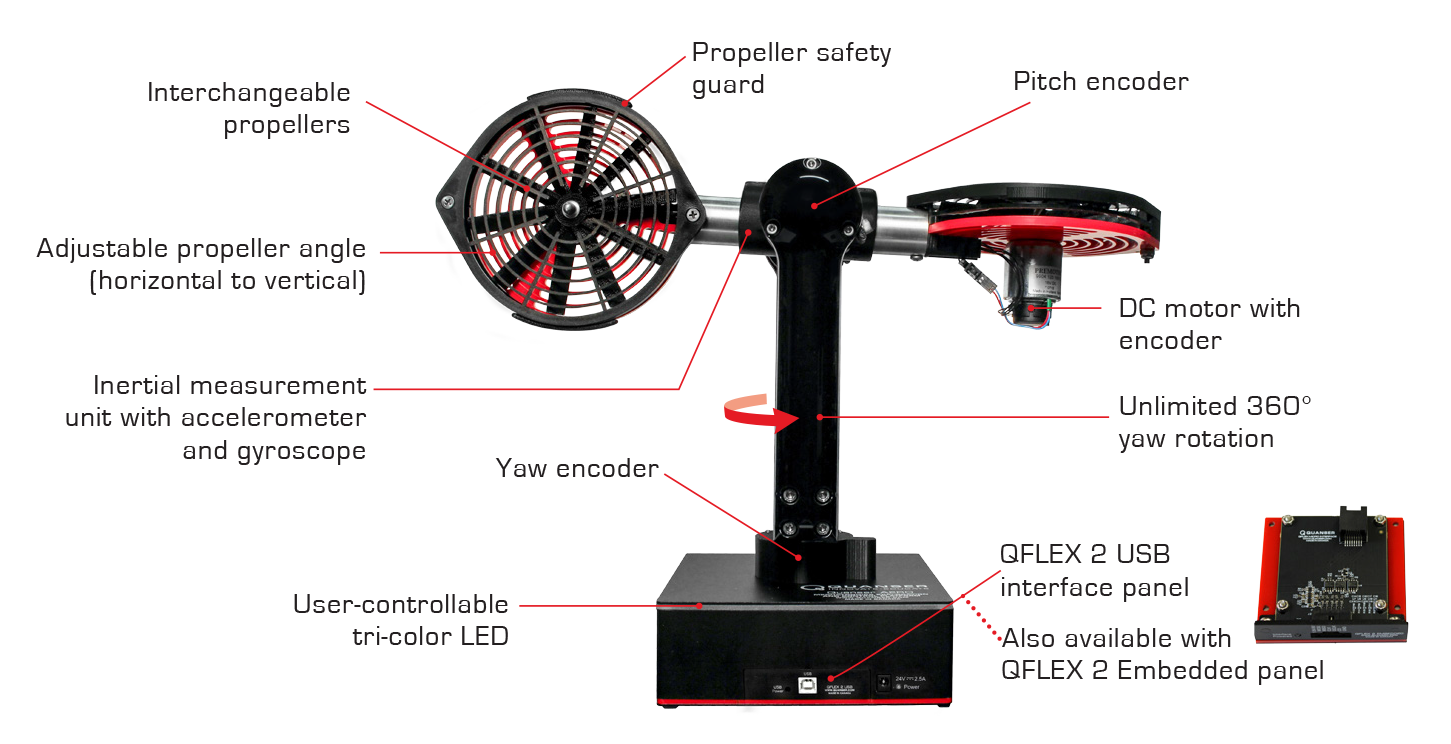
\includegraphics[width=.75\textwidth,keepaspectratio=true]{figs/img/quanserAero.png}
    \label{fig:quanserAero}
    \caption{Quanser Aero}
\end{figure}
The front rotor (horizontal to the ground) is configured to rotate about pitch axis and the tail rotor (parallel to vertical plane) is mounted to rotate about yaw axis. To measure the pitch $(\theta)$ and yaw $(\psi)$ angles, two position sensors (encoders) are mounted as shown in Fig.~\ref{fig:quanserAero}. For sake of simplicity in modeling 2-DOF helicopter, the  dynamic coupling of the Quanser Aero is omitted due to high-efficiency rotors mounted on it\footnote{See Quanser Aero user manual for details.}. The main (tail) rotor is attached to the horizontal (vertical) propeller, which is rotated by applying input voltages to corresponding DC motors. Let $v_p(v_y)$ denote the input voltage to pitch (yaw) DC motor and the state of the 2-DOF helicopter at time $t\ge 0$ is denoted by ${\bf x}^T(t) \equiv [\theta(t),\psi(t),\dot\theta(t),\dot\psi(t)],$ where $\dot\theta(\dot\psi)$ denote the rotational speed of the pitch (yaw). The free-body diagram of the 2-DOF helicopter is shown in Fig.~\ref{fig:helicopterModel}, 

\begin{figure}[!htbp]
 \begin{center}
  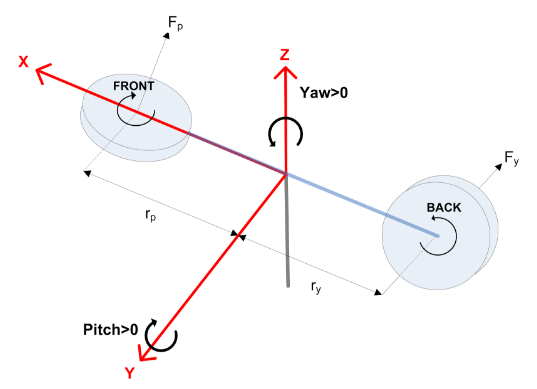
\includegraphics[scale=.75]{figs/img/helicoterModel.png}
 \end{center}
\caption{Helicopter Model}
\label{fig:helicoterModel}
\end{figure}

where $F_p(F_y)$ is force from the pitch (yaw) motor. If ${\bf u}^T(t)  \equiv [v_p(t),v_y(t)]$ denote the vector of the input voltages for DC motors at time $t\ge 0,$ then the state-space model of the 2-DOF helicopter (Quanser Aero) is described by~\cite{FaBiMi2018-c1}:
%
\begin{align}
  \dot{\bf x}(t) = {\bf A}{\bf x}(t) +{\bf B}{\bf u}(t),~\mathrm{where}
\label{eq:stateModel}
\end{align}  
%
\begin{align*}
{\bf A} =  
\begin{bmatrix}
0 & 0 & 1 & 0\\
0 & 0 & 0 & 1\\
-\frac{K_{\text{sp}}}{J_p} & 0 & -\frac{D_p}{J_p} &  0\\
0 & 0 & 0 & -\frac{D_y}{J_y}    
\end{bmatrix}
~\text{and}~
  {\bf B} =
\begin{bmatrix}
0 & 0\\
0 & 0\\
\frac{K_{\text{pp}}}{J_p} & \frac{K_{\text{py}}}{J_p}\\
\frac{K_{\text{yp}}}{J_y} & \frac{K_{\text{yy}}}{J_y}                           
\end{bmatrix},
\end{align*}
%
with $K_{sp},$ $K_{pp},$ $K_{py},$ $K_{yp},$ $K_{yy},$ $J_p,$ $J_y,$ $D_p,$ and $D_y$ being the stiffness of the axes, pitch motor thrust constant, thrust constant acting on the pitch angle from the yaw motor, thrust constant acting on yaw angle from pitch motor, yaw motor thrust constant, moment of inertia about pitch axis, moment of inertia about yaw axis, viscous damping of the pitch axis, and viscous damping of the yaw axis, respectively.\\ 
\\
In the context of a teleoperation system, a standard problem in controlling motion of states of a 2-DOF helicopter is to find optimal actuator commands $\mathbf{u}^*(t)\equiv[v_p^*(t),v_y^*(t)]^T,$ such that it follows the command signal, which is the desired (reference) state ${\bf x}^{d} = [\theta^{d},\psi^{d},0,0]^T,$ sent by the human operator through a mobile device. 




%----------------------------------------------------------------------
%\section{New Section}
%----------------------------------------------------------------------


%%% Local Variables:
%%% mode: latex
%%% TeX-master: "../finalReportMainV1"
%%% End:

%======================================================================
\chapter{Control Algorithms}
\label{ch: Chapter3}
%======================================================================
This chapter discusses the three control algorithms used in the experiment.  These are linear quadratic regulator (LQR), linear quadratic gaussian (LQG), and approximate dynamic programming (ADP).
%----------------------------------------------------------------------
\section{LQR}
%----------------------------------------------------------------------
LQR is a optimal control algorithm that is used to calculate the control gain.\\
    After creating the system model
    \begin{align*}
        \dot{\mathbf{x}} = \mathbf{A}\mathbf{x} + \mathbf{B}\mathbf{u}
    \end{align*}
    use the state feedback law
    \begin{center}
        $\mathbf{u} = -\mathbf{K}\mathbf{x}$
    \end{center}
    to minimize the quadratic cost function:
    \begin{align*}
        J(\mathbf{u}) = \int_0^\infty (\mathbf{x}^T\mathbf{Q}\mathbf{x} + \mathbf{u}^T\mathbf{R}\mathbf{u} + 2\mathbf{x}^T\mathbf{N}\mathbf{u})\mathrm{dt}
    \end{align*}
    Find the solution $\mathbf{S}$ to the Riccati equation
    \begin{align*}
        \mathbf{A}^T\mathbf{S}+\mathbf{SA}-(\mathbf{SB}+\mathbf{N})\mathbf{R}^{-1}(\mathbf{B}^T\mathbf{S}+\mathbf{N}^T)+\mathbf{Q}=0
    \end{align*}    
    Calculate gain, $\mathbf{K}$
    \begin{center}
        $\mathbf{K}=\mathbf{R}^{-1}(\mathbf{B}^T\mathbf{S}+\mathbf{N}^T)$
    \end{center}

%----------------------------------------------------------------------
\section{LQG}
%----------------------------------------------------------------------
LQG utilizes gain calculated in LQR but it adds a Kalman filter to reduce external disturbances to the system.


%----------------------------------------------------------------------
\section{ADP}
%----------------------------------------------------------------------
ADP is a reienforcement learning approach.  It utilizes the error of the state variables and feeds them into a hidden layer of neurons as shown in Figrure~\ref{fig:ADP_Neural_Network}.  Each of these neuron uses a quadratic activation function which is a function of error.  The result of these nodes are mutiplied by a weight which is then sent to an output node where they are summed.  This value is then used to calculate the control gain. 
\begin{figure}[!htbp]
    \centering
    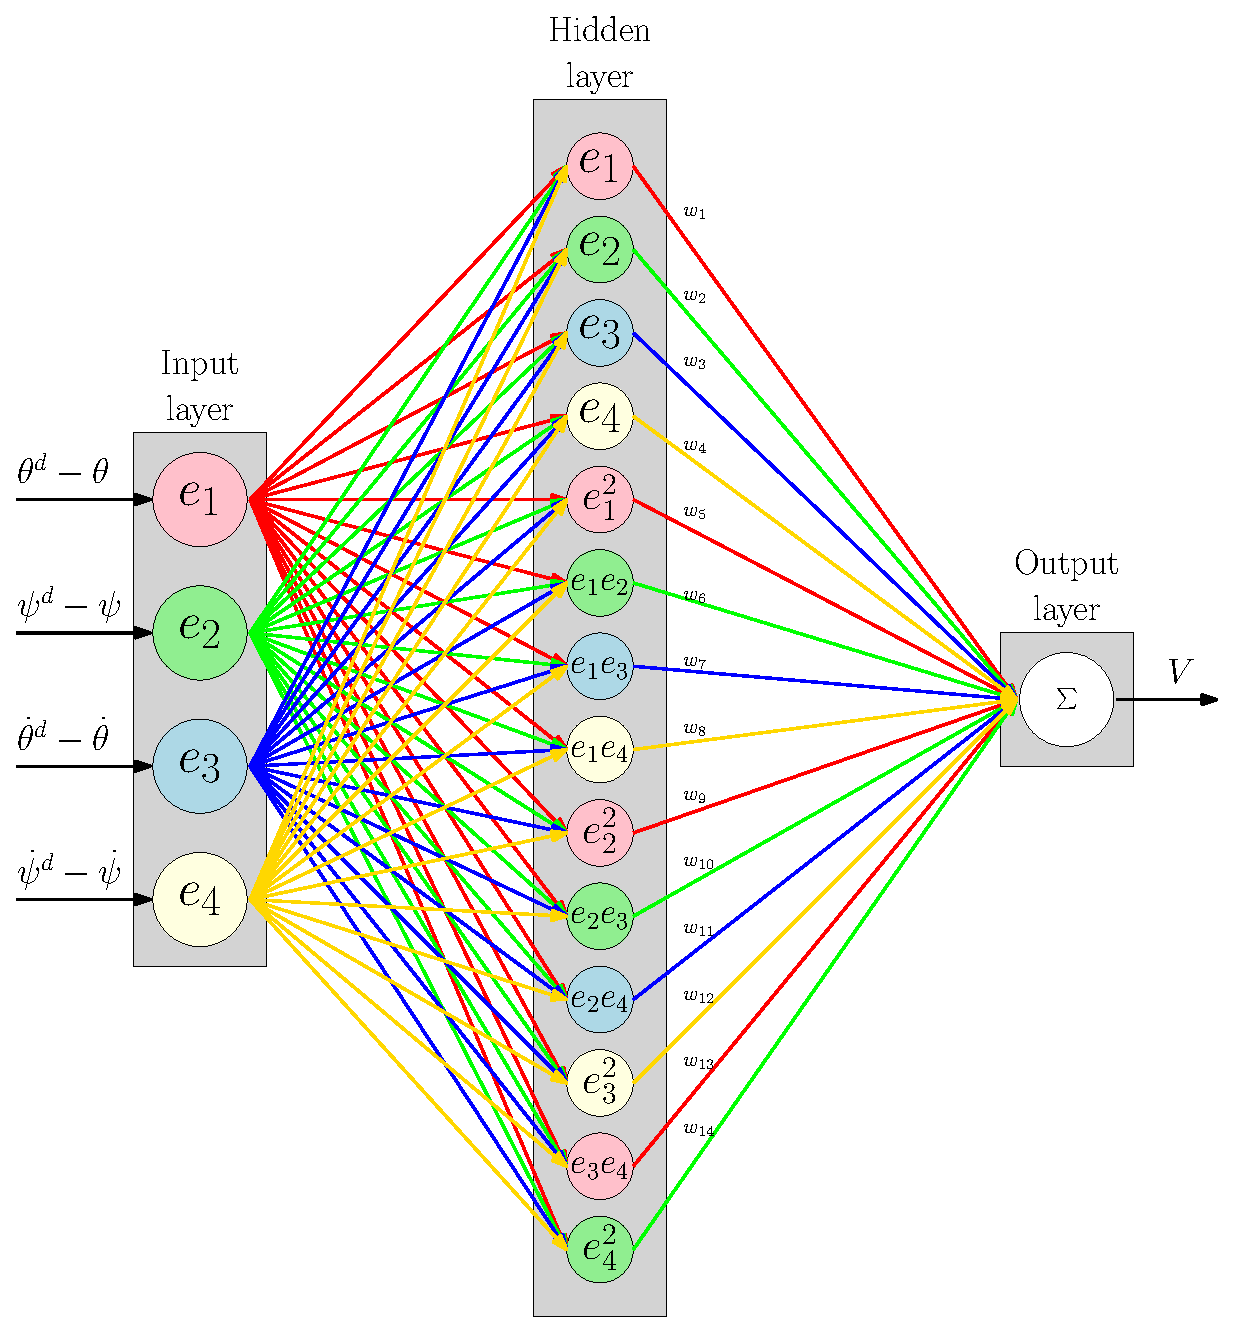
\includegraphics[width=.46\textwidth,keepaspectratio=true]{figs/ipe/ADP_Neural_Network.eps}
    \caption{Input nodes are connected to the hidden layer and then to the output layer.}
    \label{fig:ADP_Neural_Network}
\end{figure}
While the system is running, the controller is collects data every $\tau$ seconds as shown in Figure~\ref{fig:ADP_Samples}.  After $T$ seconds, the data is then fed back into the neural network where the weights are updated.
\begin{figure}[!htbp]
    \centering
    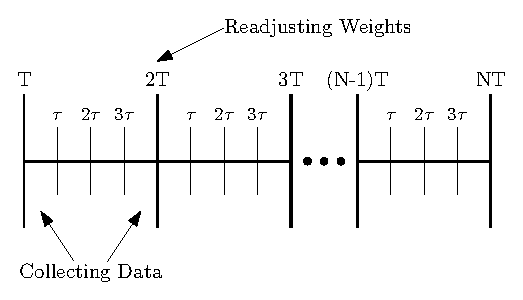
\includegraphics[width=.46\textwidth,keepaspectratio=true]{figs/ipe/ADP_Samples.eps}
    \caption{Data is collected for every $\tau$ seconds and then the weights are adjusted every $T$ seconds.}
    \label{fig:ADP_Samples}
\end{figure}

%----------------------------------------------------------------------
\section{Improvements}
Most of these algorithms are typically implemented only using proportional gain which causes steady-state error to certain input signals in some systems.  In our case, we experience steady-state error for a step input.  To reduce this, the type of the controller needs to be increased by adding an integrator.  We solve this problem by implementing a PI controller where LQR and ADP are used to find the optimal proportional and integral gain.\\
This is done by creating a new state varible to the system which will represent the integrated state.   As a result, the A and B will need to be augmented matrix with different dimensions.  This will also result in a different dimension of the K matrix.  The K matrix will nedd to be seperated into proportional and integral gain.

%----------------------------------------------------------------------



%%% Local Variables:
%%% mode: latex
%%% TeX-master: "../finalReport"
%%% End:

%======================================================================
\chapter{Numerical Simulations}
%\chapter{MATLAB Simulations}
\label{ch: Chapter4}
%======================================================================

%----------------------------------------------------------------------
\section{LQR (P controller)}
%----------------------------------------------------------------------
Using MATLAB, we created a program, as seen in \ref{ch:codeLQRsim}, that calculates LQR for our helicopter and then uses differential equations to simulate the trajectory. \ref{fig:LQR_Pos_Con} \ref{fig:LQR_Error_Con}  \ref{fig:LQR_Volt_Con}  

\begin{figure}[!htbp]
    \centering
    \subfigure[][]{
    %\missingfigure{Insert figure.}
    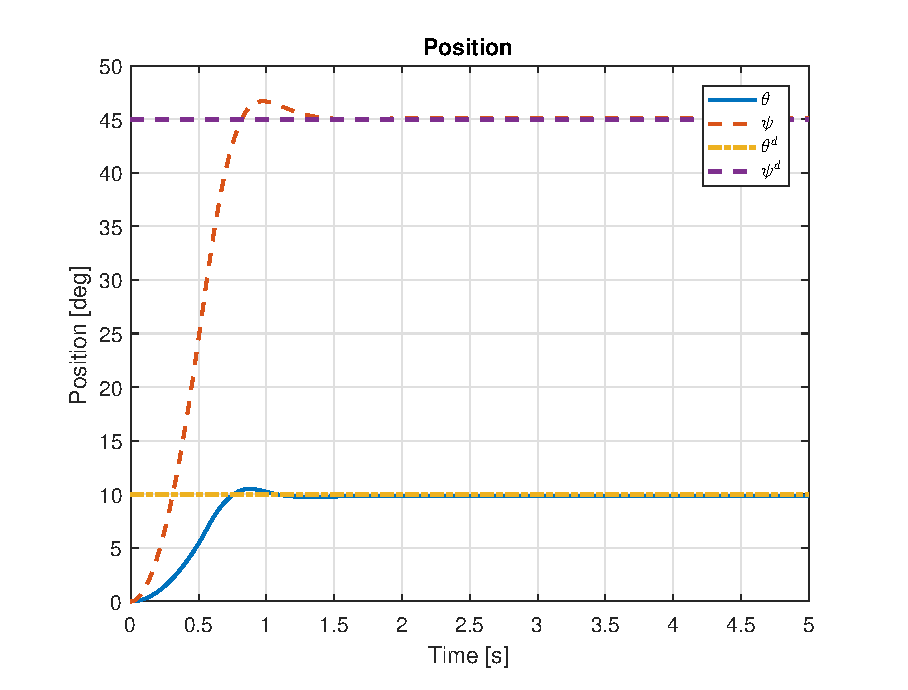
\includegraphics[width=.46\textwidth,keepaspectratio=true]{figs/matlab/LQR/P_Simulation/LQR_Pos_Con.eps}
    \label{fig:LQR_Pos_Con}
    }
    \subfigure[][]{
    %\missingfigure{Insert figure.}
    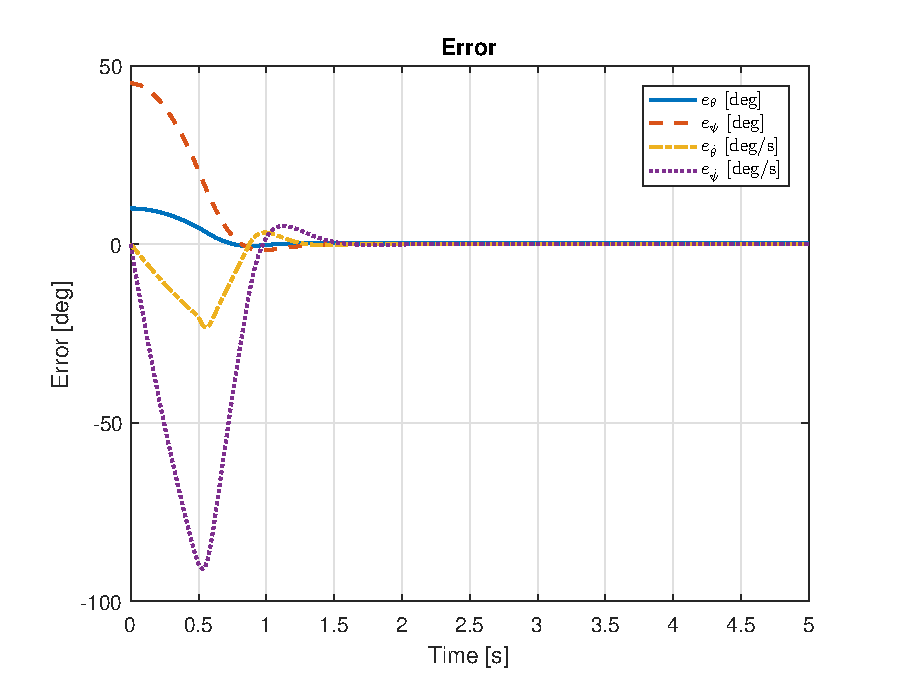
\includegraphics[width=.46\textwidth,keepaspectratio=true]{figs/matlab/LQR/P_Simulation/LQR_Error_Con.eps}
    \label{fig:LQR_Error_Con}
    }
    \subfigure[][]{
    %\missingfigure{Insert figure.}
    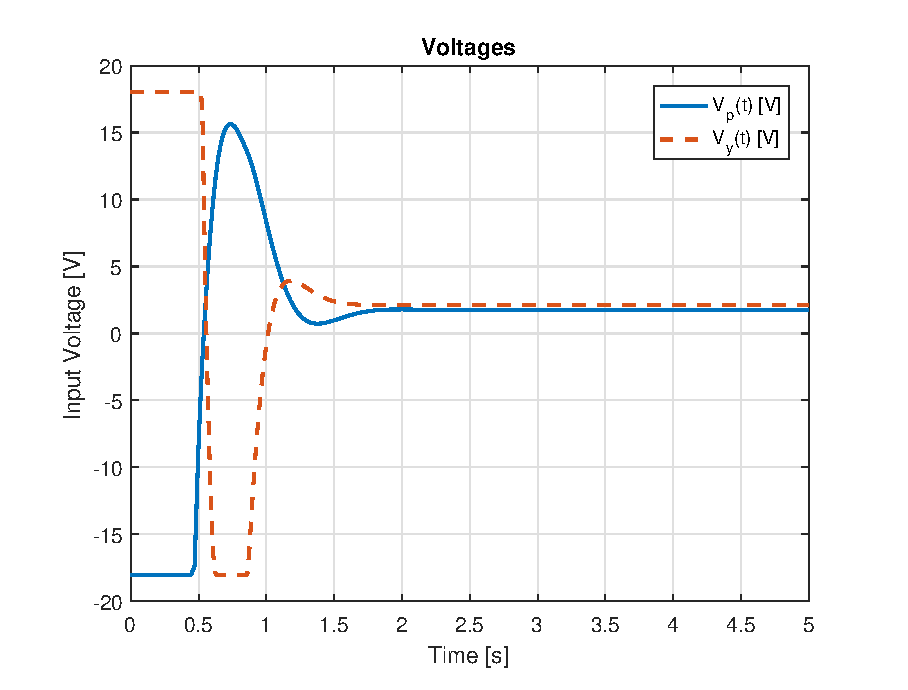
\includegraphics[width=.46\textwidth,keepaspectratio=true]{figs/matlab/LQR/P_Simulation/LQR_Volt_Con.eps}
    \label{fig:LQR_Volt_Con}
    }
    \caption{Simulations for proportional gain calculated by LQR.}
\end{figure}

%----------------------------------------------------------------------
\section{LQR (PI controller)}
%----------------------------------------------------------------------
\todo[inline]{Insert Block diagram for LQR PI simulation}
%\todo[inline]{Insert results for LQR PI simulation}
\begin{figure}[!htbp]
    \centering
    \subfigure[][]{
    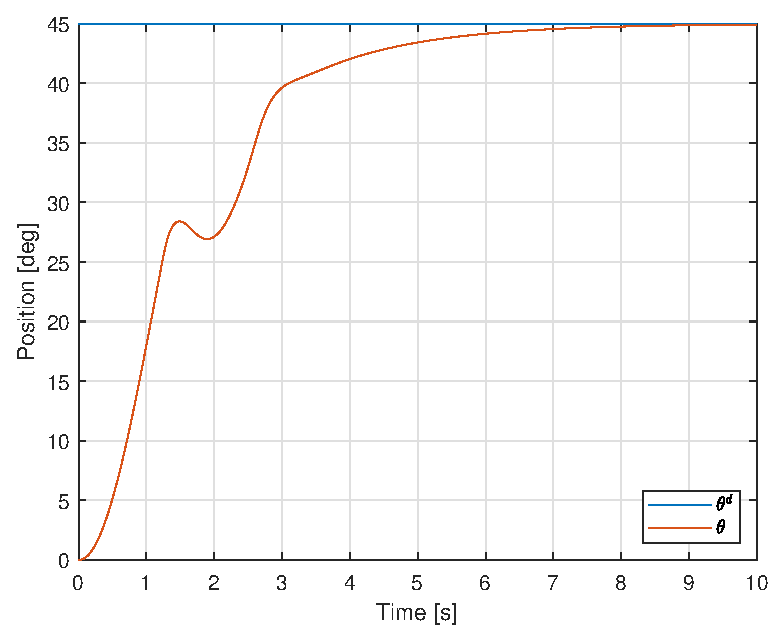
\includegraphics[width=.46\textwidth,keepaspectratio=true]{figs/matlab/LQR/PI_Sim/Pitch_LQR_Sim.eps}
    \label{fig:Pitch_LQR_Sim}
    }
    \subfigure[][]{
    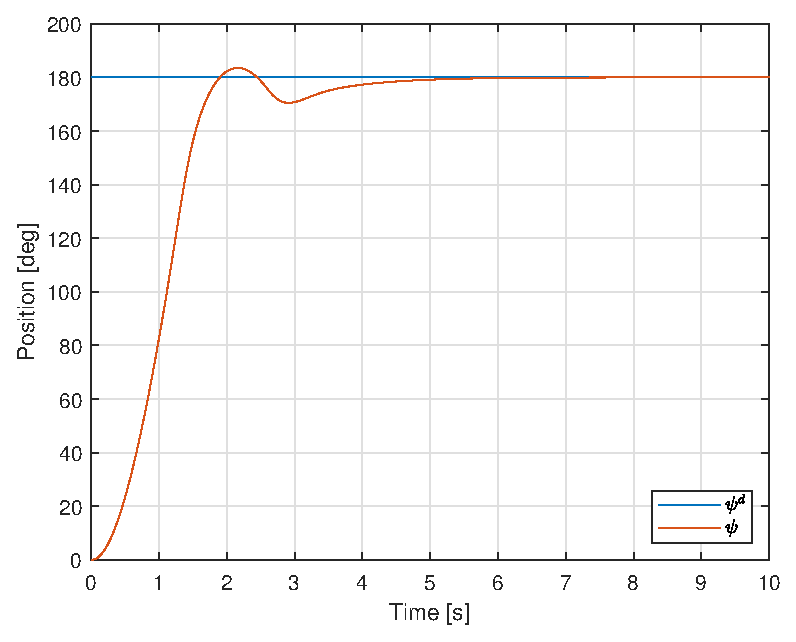
\includegraphics[width=.46\textwidth,keepaspectratio=true]{figs/matlab/LQR/PI_Sim/Yaw_LQR_Sim.eps}
    \label{fig:Yaw_LQR_Sim}
    }    
    \subfigure[][]{
    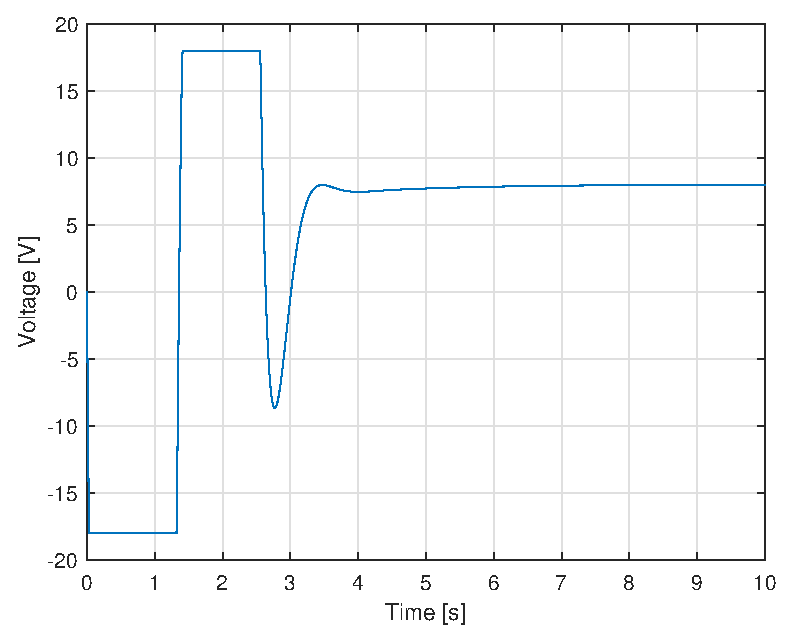
\includegraphics[width=.46\textwidth,keepaspectratio=true]{figs/matlab/LQR/PI_Sim/Pitch_Volt_LQR_Sim.eps}
    \label{fig:Pitch_Volt_LQR_Sim}
    }    
    \subfigure[][]{
    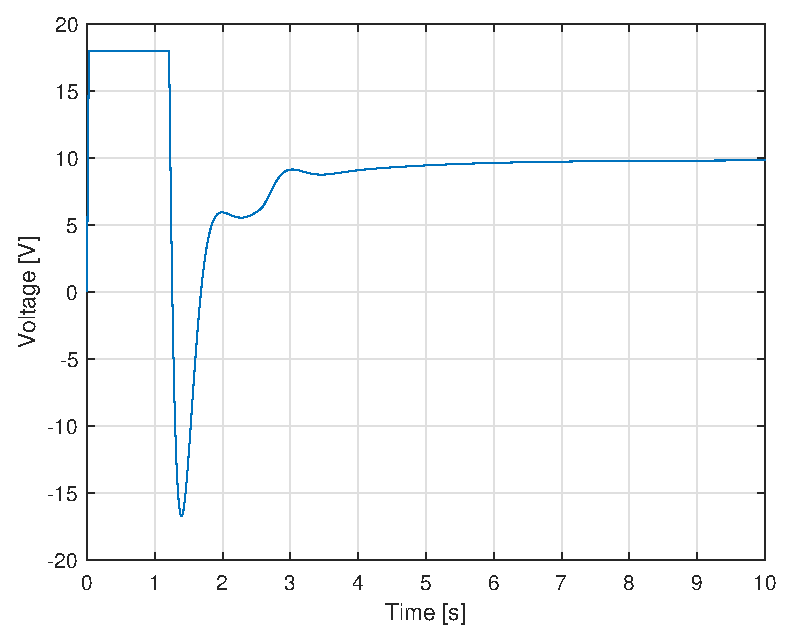
\includegraphics[width=.46\textwidth,keepaspectratio=true]{figs/matlab/LQR/PI_Sim/Yaw_Volt_LQR_Sim.eps}
    \label{fig:Yaw_Volt_LQR_Sim}
    }
    \caption{Simulations for proportional and integral gain calculated by LQR.}
\end{figure}

%----------------------------------------------------------------------
\section{LQG (PI Controller)}
%----------------------------------------------------------------------
\todo[inline]{Insert Block diagram for LQG PI simulation}
%\todo[inline]{Insert results for LQG PI simulation}
\begin{figure}[!htbp]
    \centering
    \subfigure[][]{
    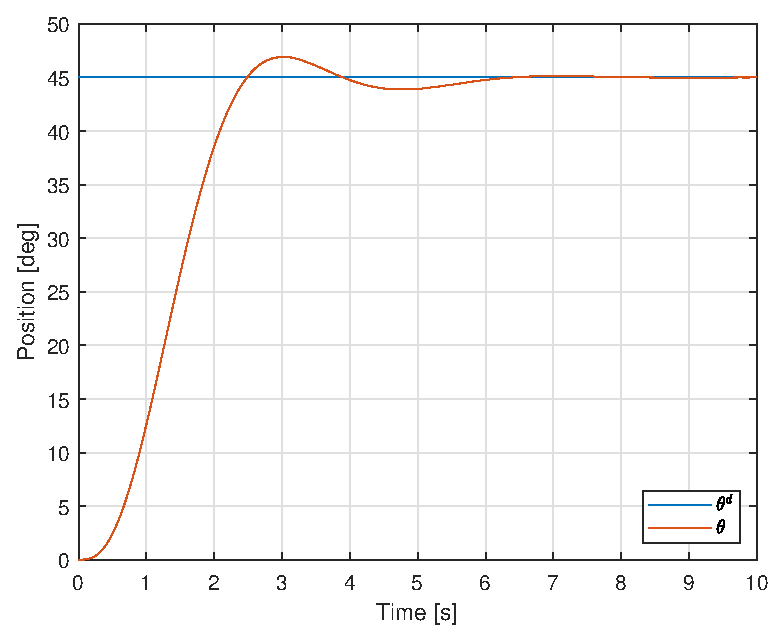
\includegraphics[width=.46\textwidth,keepaspectratio=true]{figs/matlab/LQG/LQG_Sim/Pitch_LQG_Sim.eps}
    \label{fig:Pitch_LQG_Sim}
    }
    \subfigure[][]{
    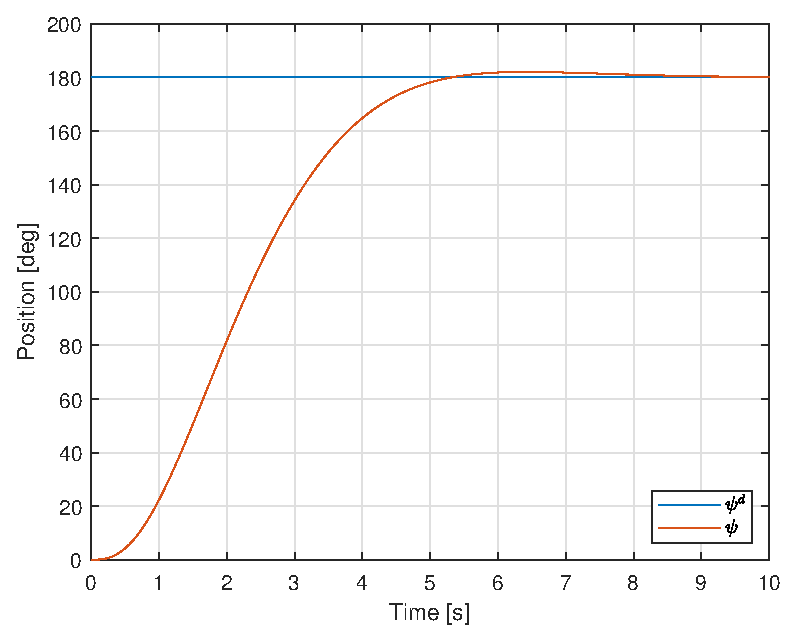
\includegraphics[width=.46\textwidth,keepaspectratio=true]{figs/matlab/LQG/LQG_Sim/Yaw_LQG_Sim.eps}
    \label{fig:Yaw_LQG_Sim}
    }    
    \subfigure[][]{
    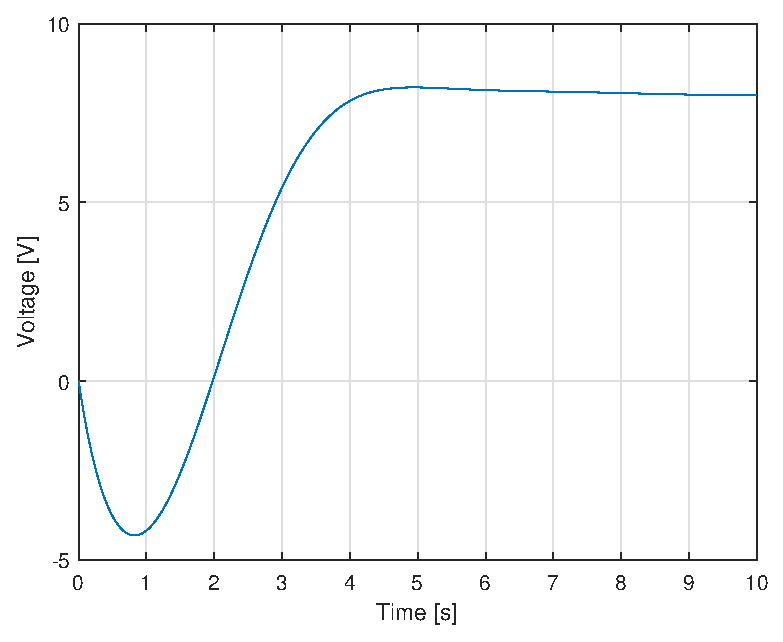
\includegraphics[width=.46\textwidth,keepaspectratio=true]{figs/matlab/LQG/LQG_Sim/Pitch_Volt_LQG_Sim.eps}
    \label{fig:Pitch_Volt_LQG_Sim}
    }    
    \subfigure[][]{
    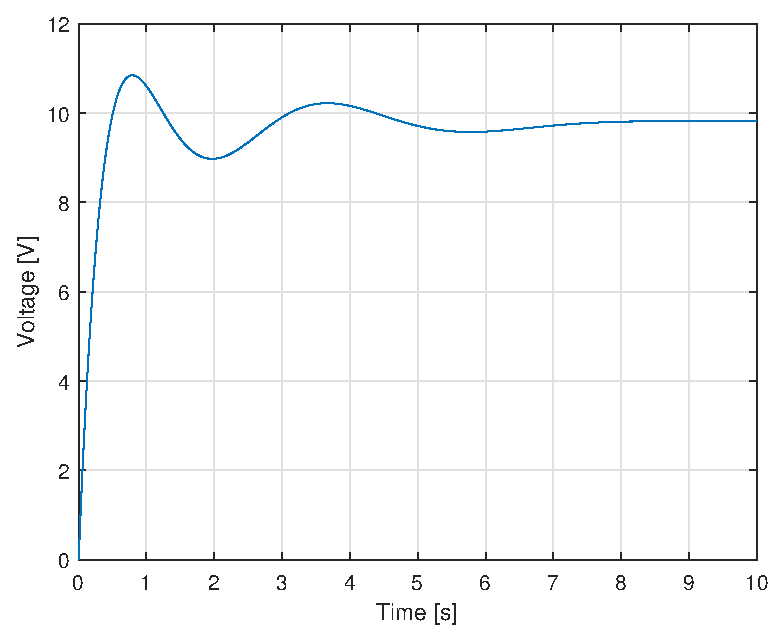
\includegraphics[width=.46\textwidth,keepaspectratio=true]{figs/matlab/LQG/LQG_Sim/Yaw_Volt_LQG_Sim.eps}
    \label{fig:Yaw_Volt_LQG_Sim}
    }
    \caption{Simulations for proportional and integral gain calculated by LQG.}
\end{figure}

%----------------------------------------------------------------------
\section{Conclusions}
%----------------------------------------------------------------------
Note: constant used pitch XXXX degrees, yaw XXXX degrees\\
Note: square used pitch XXXX degrees with period of XXXX, yaw XXXX degrees with period of XXXX\\
Note: sine used pitch XXXX degrees with period of XXXX, yaw XXXX degrees with period of XXXX\\
\begin{table}[!htbp]
    \centering
    \begin{tabular}{l|l|l|l|l|l|l}
        \toprule
        \textbf{} & \textbf{LQR(P)} & \textbf{LQR(PI)} & \textbf{LQG(PI)} \\
        \toprule
        RMSE Pitch Step & ? & ? & ?  \\
        RMSE Yaw Step & ? & ? & ? \\
        RMSE Pitch Square & ? & ? & ? \\
        RMSE Yaw Square & ? & ? & ? \\
        RMSE Pitch Sine & ? & ? & ? \\
        RMSE Yaw Sine & ? & ? & ? \\
        \bottomrule
    \end{tabular}
    \caption{Error Comparison for Simulated Algorithms}
    \label{tab:Simulate_RMSE}
\end{table}
Based on the results XXXX preformed better in the simulations.
%----------------------------------------------------------------------



%%% Local Variables:
%%% mode: latex
%%% TeX-master: "../finalReport"
%%% End:

%======================================================================
\chapter{Implementation}
\label{ch: Chapter5}
%======================================================================

%======================================================================
\section{Experimental Setup}
%----------------------------------------------------------------------
\subsection{USB}
%----------------------------------------------------------------------


%----------------------------------------------------------------------
\subsection{Raspberry Pi}
%----------------------------------------------------------------------
The communication protocol utilized by the Q-Flex2 embedded panel is SPI.  
\begin{figure}[!htbp]
    \centering
    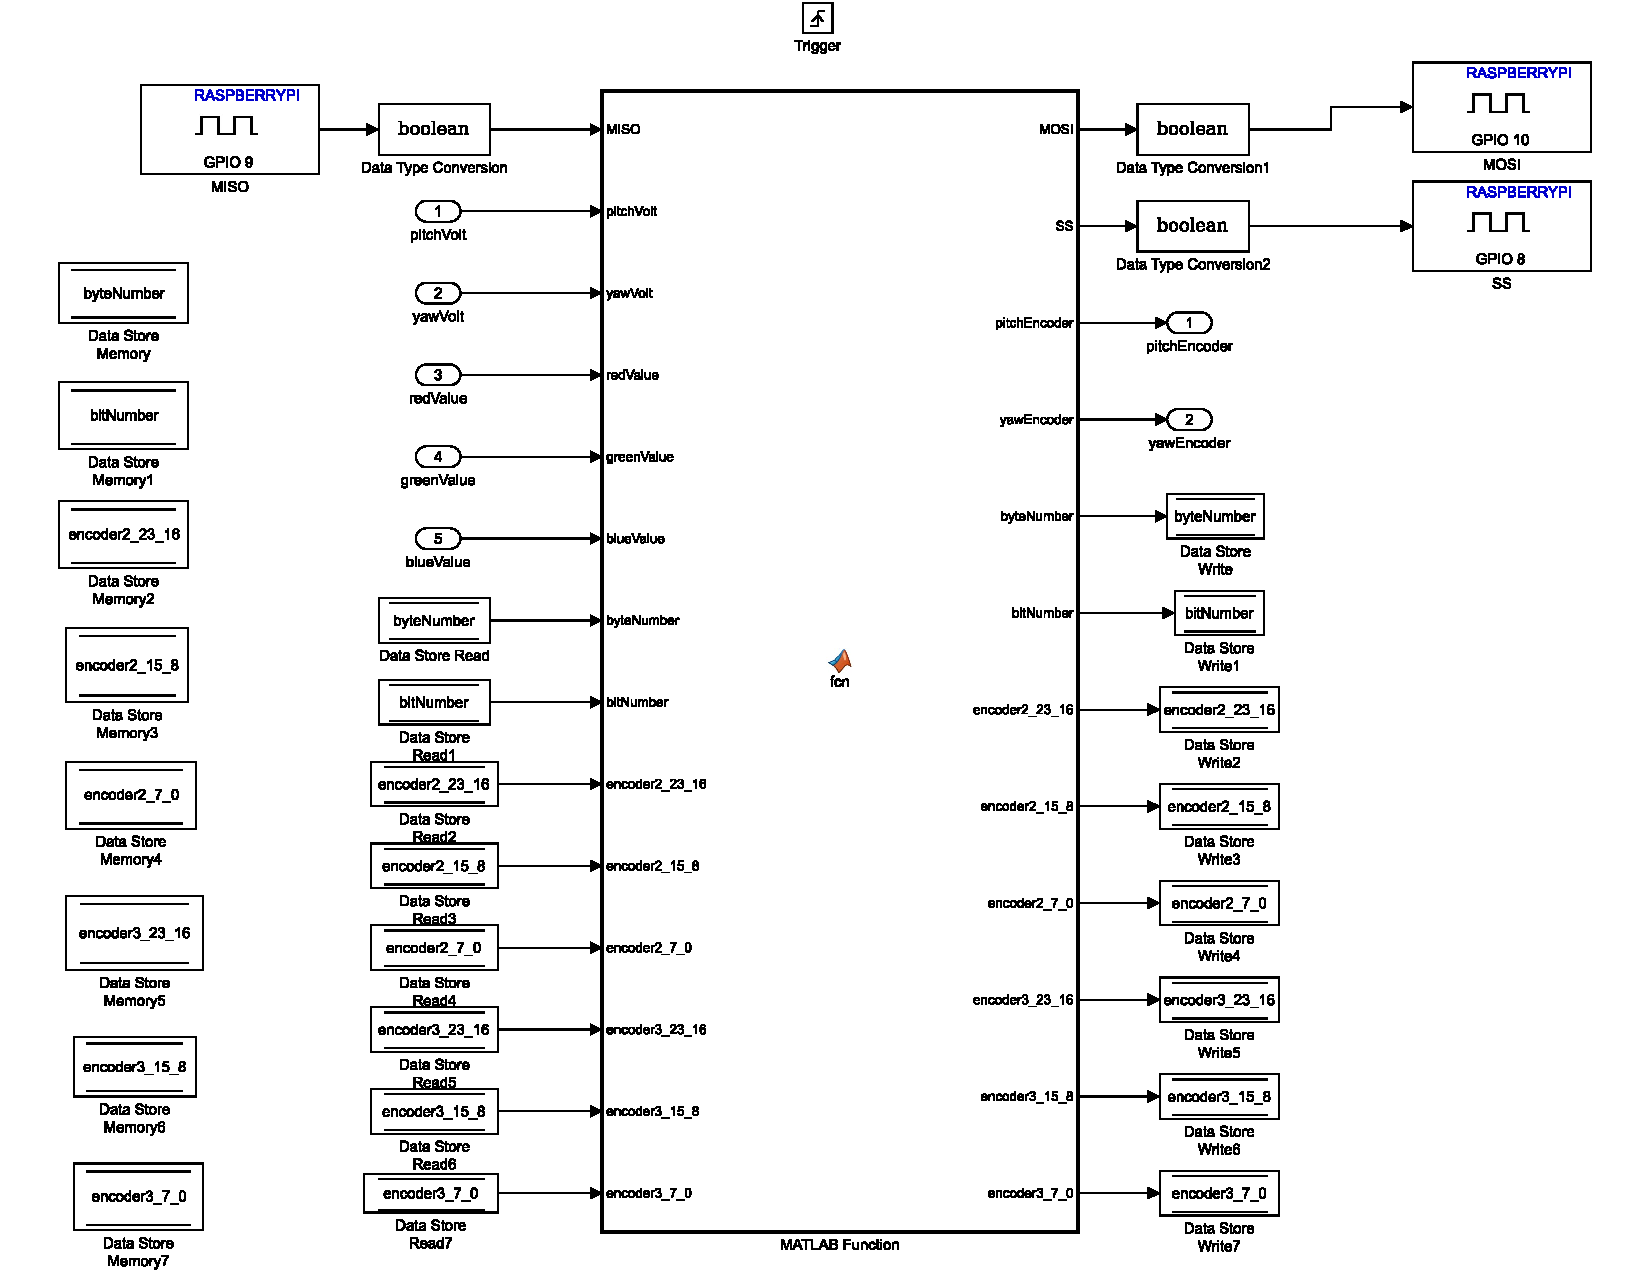
\includegraphics[width=.46\textwidth,keepaspectratio=true]{figs/img/SPI_COM.pdf}
    \label{fig:SPI_COM}
    \caption{Block diagram of SPI communication protocol used for communication between the Raspberry Pi and Quanser Aero.}
\end{figure}


%----------------------------------------------------------------------
\subsection{Android}
%----------------------------------------------------------------------
\begin{figure}[!htbp]
    \centering
    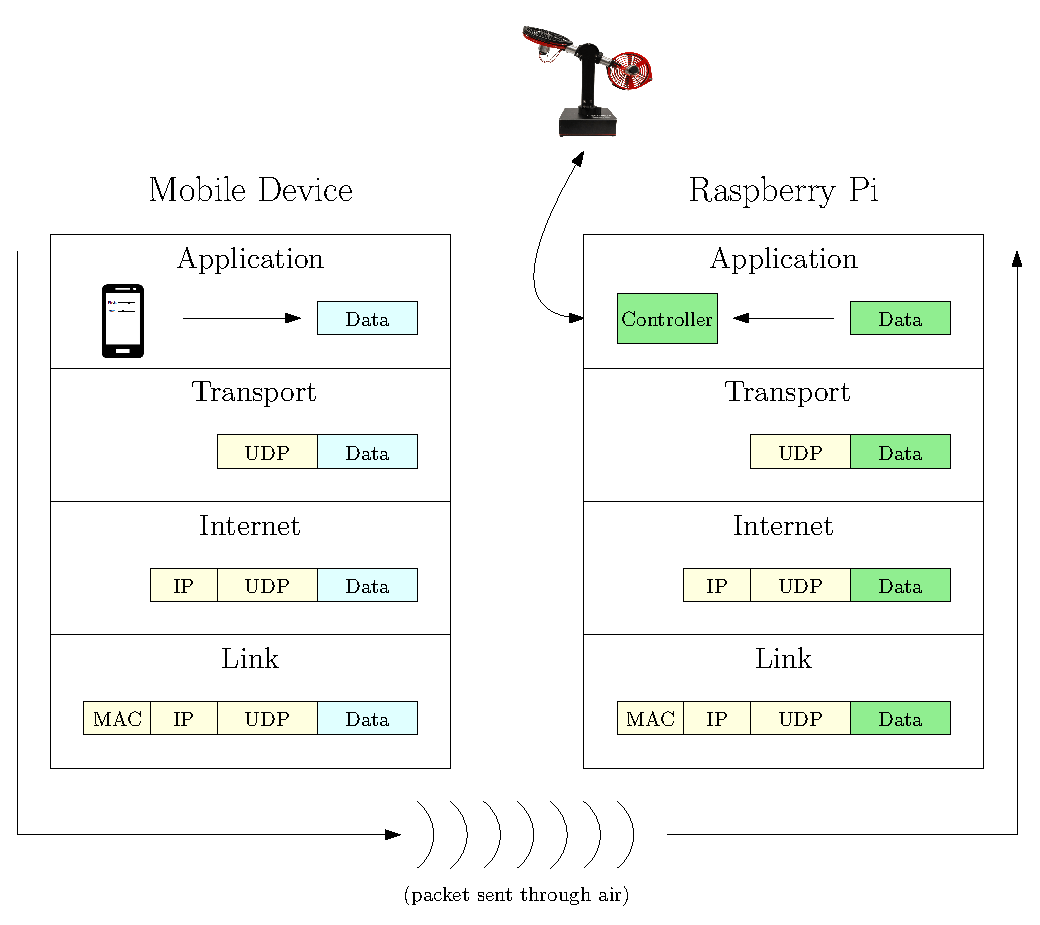
\includegraphics[width=.46\textwidth,keepaspectratio=true]{figs/ipe/TCPModel.eps}
    \label{fig:TCPModel}
    \caption{Illustration of the TCP model which describes how packets are sent and recieved from mobile devices to the Quanser Aero.}
\end{figure}

\begin{figure}[!htbp]
    \centering
    \includegraphics[width=.5\textwidth,keepaspectratio=true]{figs/ipe/Setup.eps}
    \label{fig:Setup}
    \caption{Experiment setup for controlling the Quanser Aeros via a mobile device.}
\end{figure}

%======================================================================
\section{USB}
%----------------------------------------------------------------------
\subsection{LQR}
%----------------------------------------------------------------------

\begin{figure}[!htbp]
    \centering
    \subfigure[][]{
    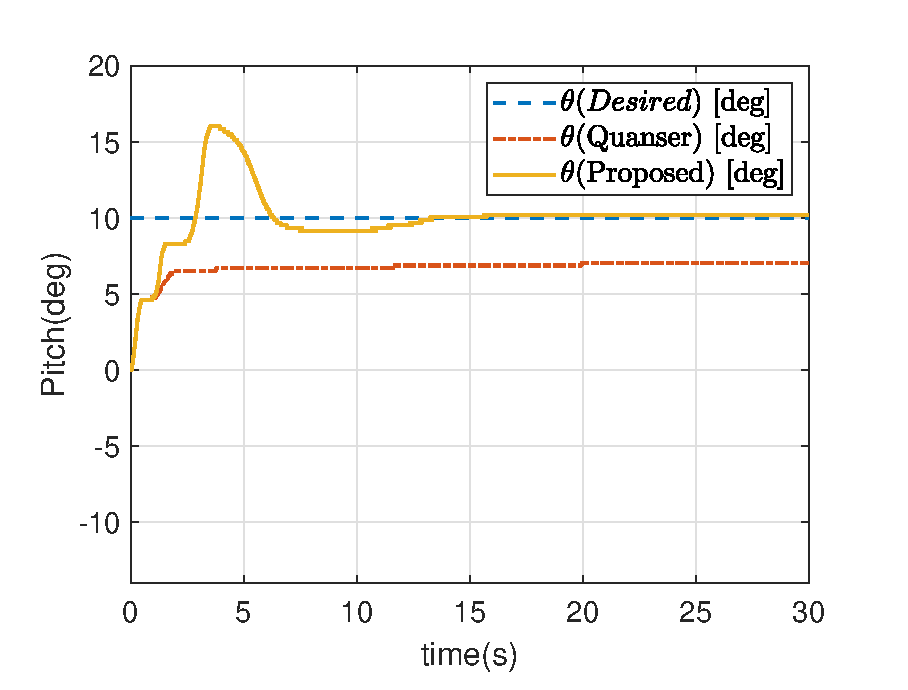
\includegraphics[width=.46\textwidth,keepaspectratio=true]{figs/matlab/LQR_PIvLQR_P_USB/step/Pitch_LQR_RMSE.eps}
    \label{fig:Pitch_LQR_RMSE_Step}
    }
    \subfigure[][]{
    \includegraphics[width=.46\textwidth,keepaspectratio=true]{figs/matlab/LQR_PIvLQR_P_USB/step/Yaw_LQR_RMSE.eps}
    \label{fig:Yaw_LQR_RMSE_Step}
    }    
    \subfigure[][]{
    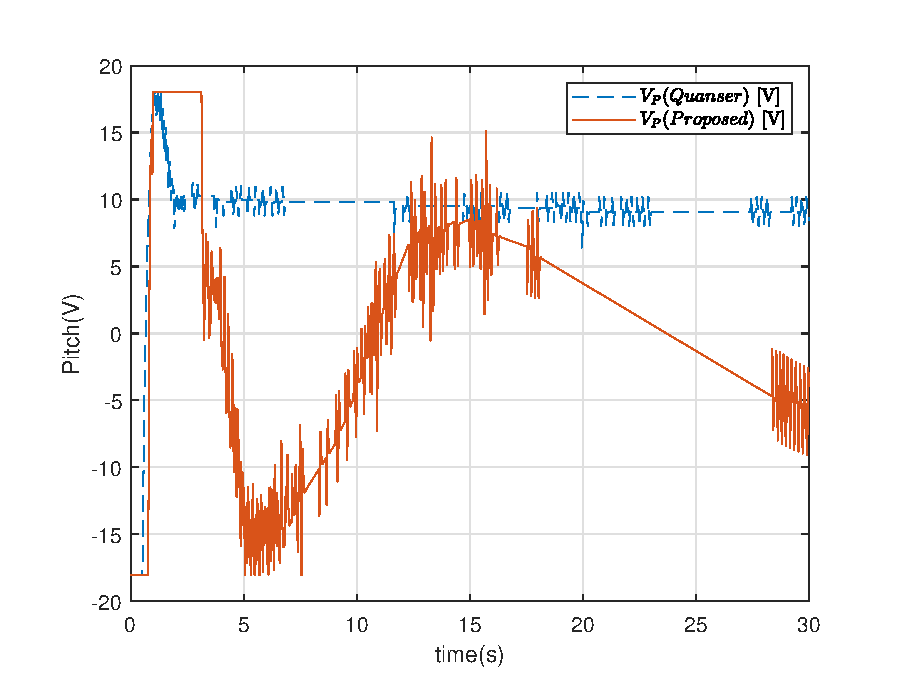
\includegraphics[width=.46\textwidth,keepaspectratio=true]{figs/matlab/LQR_PIvLQR_P_USB/step/PitchVoltage_LQR_RMSE.eps}
    \label{fig:PitchVoltage_LQR_RMSE_Step}
    }    
    \subfigure[][]{
    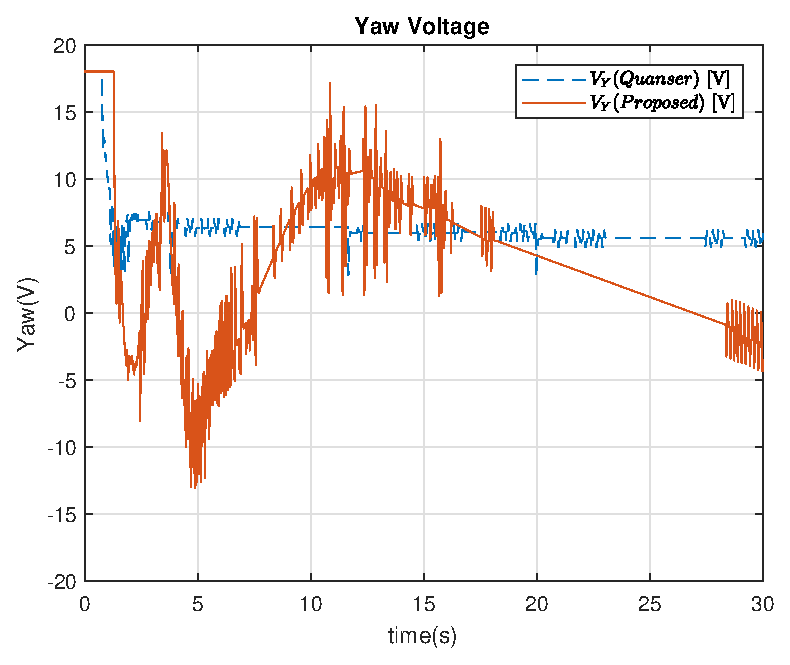
\includegraphics[width=.46\textwidth,keepaspectratio=true]{figs/matlab/LQR_PIvLQR_P_USB/step/YawVoltage_LQR_RMSE.eps}
    \label{fig:YawVoltage_LQR_RMSE_Step}
    }
    \subfigure[][]{
    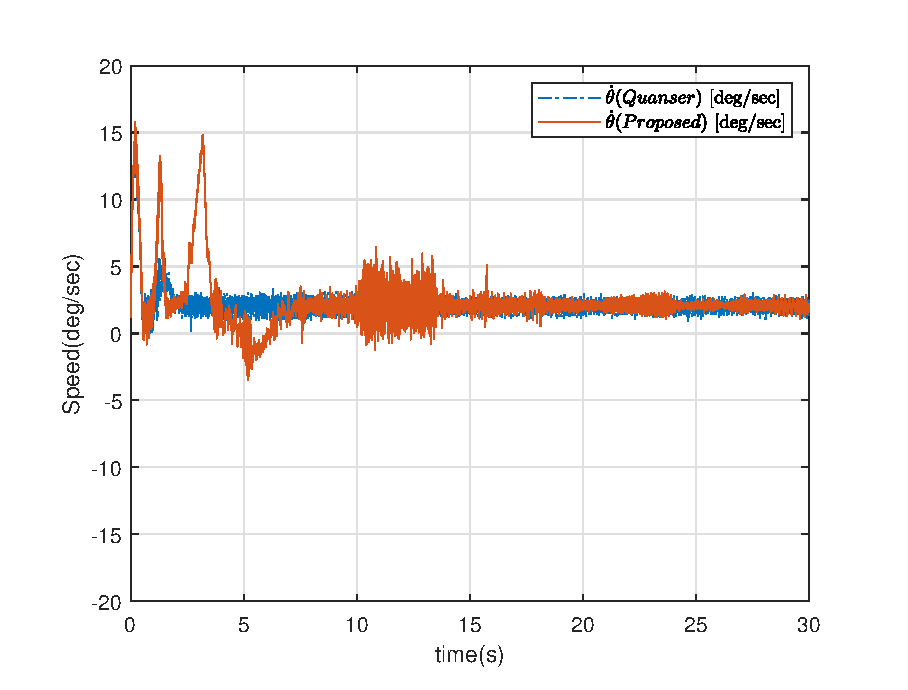
\includegraphics[width=.46\textwidth,keepaspectratio=true]{figs/matlab/LQR_PIvLQR_P_USB/step/PitchSpeed_LQR_RMSE.eps}
    \label{fig:PitchSpeed_LQR_RMSE_Step}
    }
    \subfigure[][]{
    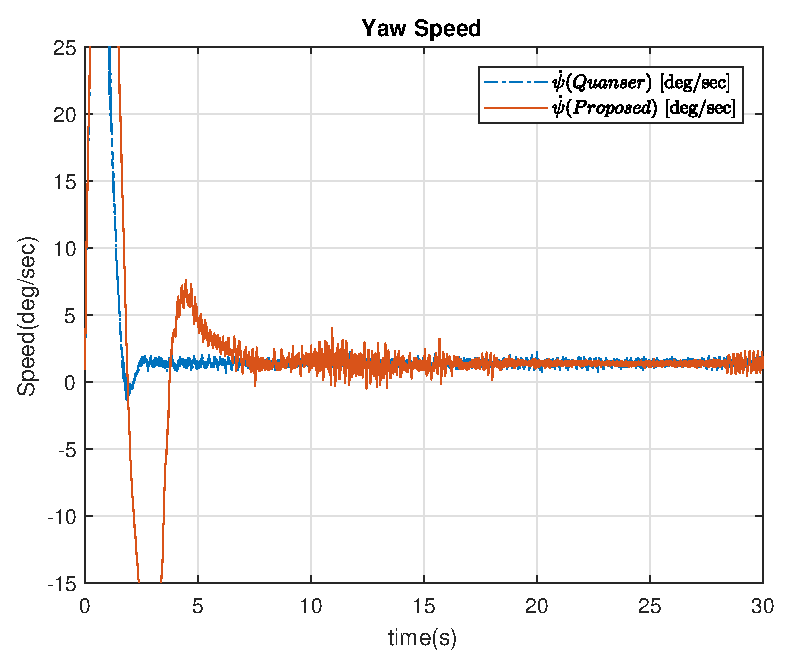
\includegraphics[width=.46\textwidth,keepaspectratio=true]{figs/matlab/LQR_PIvLQR_P_USB/step/YawSpeed_LQR_RMSE.eps}
    \label{fig:PitchSpeed_LQR_RMSE_Step}
    }
    \caption{USB implementation for proportional controller and proportional-integral controller calculated by LQR with a step input.}
\end{figure}

\begin{figure}[!htbp]
    \centering
    \subfigure[][]{
    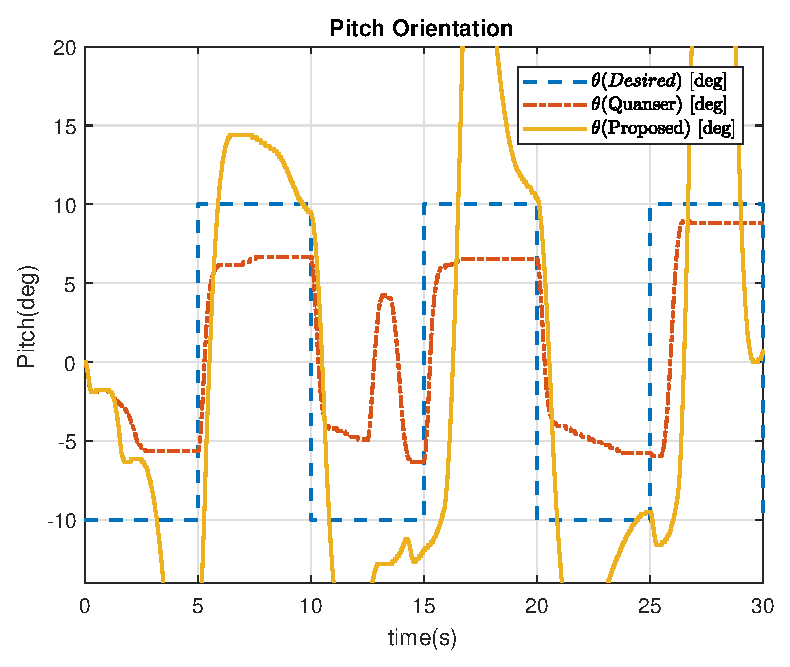
\includegraphics[width=.46\textwidth,keepaspectratio=true]{figs/matlab/LQR_PIvLQR_P_USB/square/Pitch_LQR_RMSE.eps}
    \label{fig:Pitch_LQR_RMSE_Square}
    }
    \subfigure[][]{
    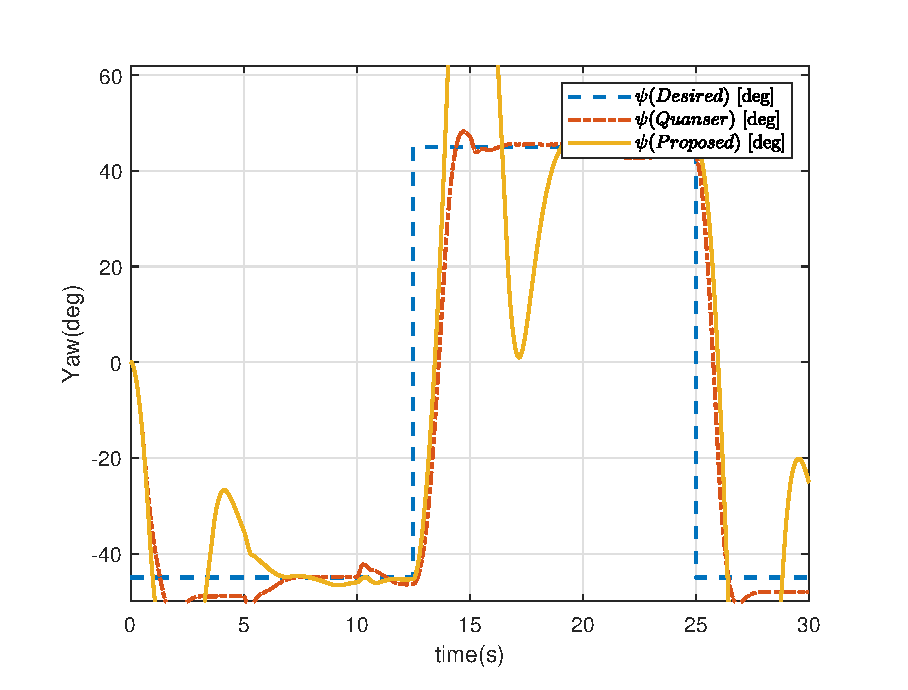
\includegraphics[width=.46\textwidth,keepaspectratio=true]{figs/matlab/LQR_PIvLQR_P_USB/square/Yaw_LQR_RMSE.eps}
    \label{fig:Yaw_LQR_RMSE_Square}
    }    
    \subfigure[][]{
    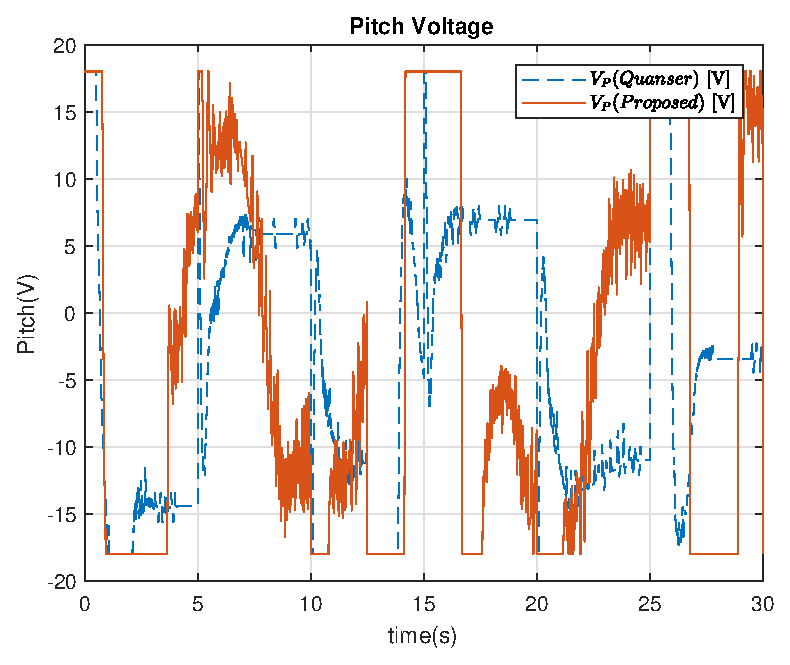
\includegraphics[width=.46\textwidth,keepaspectratio=true]{figs/matlab/LQR_PIvLQR_P_USB/square/PitchVoltage_LQR_RMSE.eps}
    \label{fig:PitchVoltage_LQR_RMSE_Square}
    }    
    \subfigure[][]{
    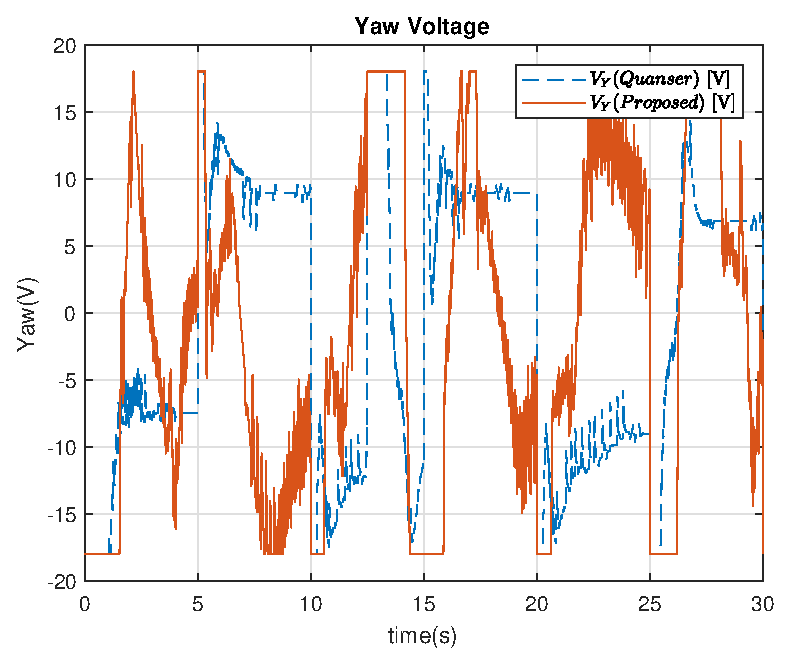
\includegraphics[width=.46\textwidth,keepaspectratio=true]{figs/matlab/LQR_PIvLQR_P_USB/square/YawVoltage_LQR_RMSE.eps}
    \label{fig:YawVoltage_LQR_RMSE_Square}
    }
    \subfigure[][]{
    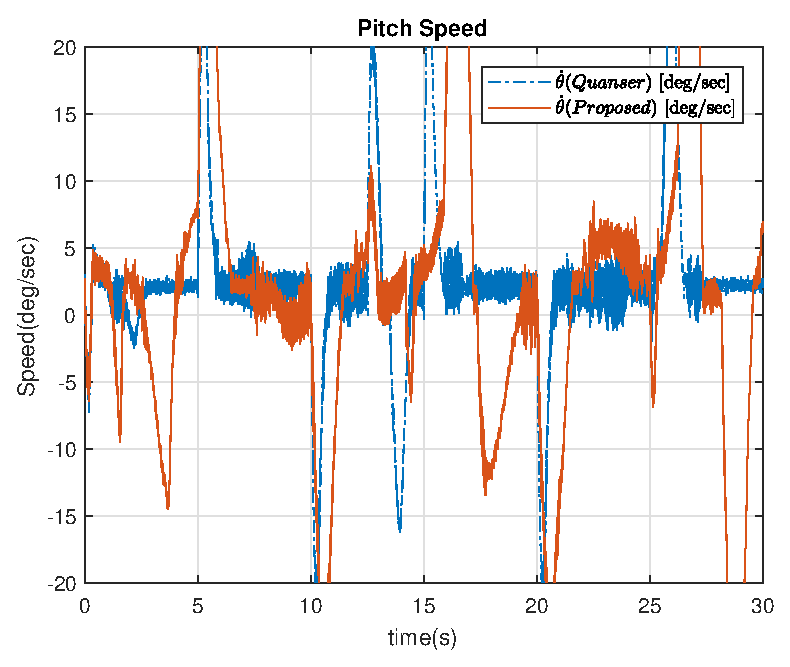
\includegraphics[width=.46\textwidth,keepaspectratio=true]{figs/matlab/LQR_PIvLQR_P_USB/square/PitchSpeed_LQR_RMSE.eps}
    \label{fig:PitchSpeed_LQR_RMSE_Square}
    }
    \subfigure[][]{
    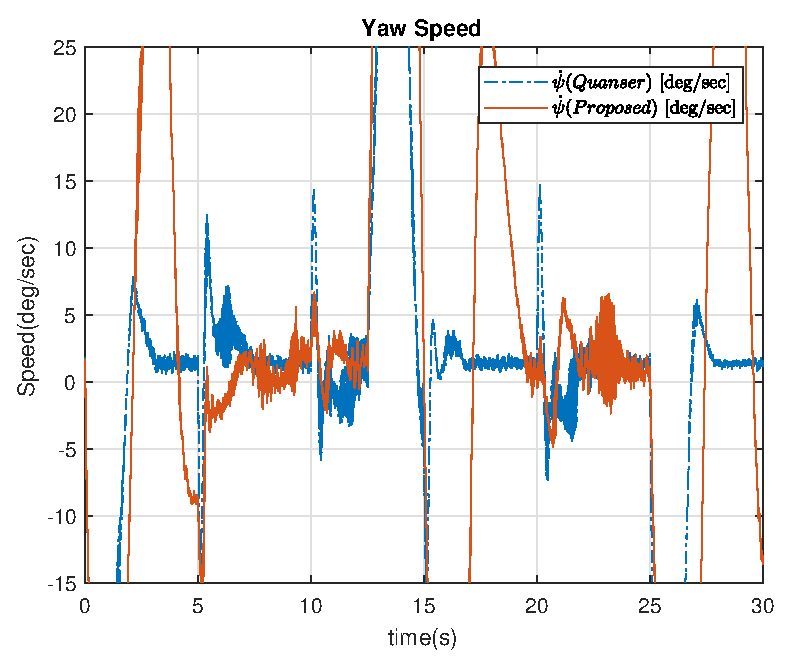
\includegraphics[width=.46\textwidth,keepaspectratio=true]{figs/matlab/LQR_PIvLQR_P_USB/square/YawSpeed_LQR_RMSE.eps}
    \label{fig:PitchSpeed_LQR_RMSE_Square}
    }
    \caption{USB implementation for proportional controller and proportional-integral controller calculated by LQR with a square wave input.}
\end{figure}

\begin{figure}[!htbp]
    \centering
    \subfigure[][]{
    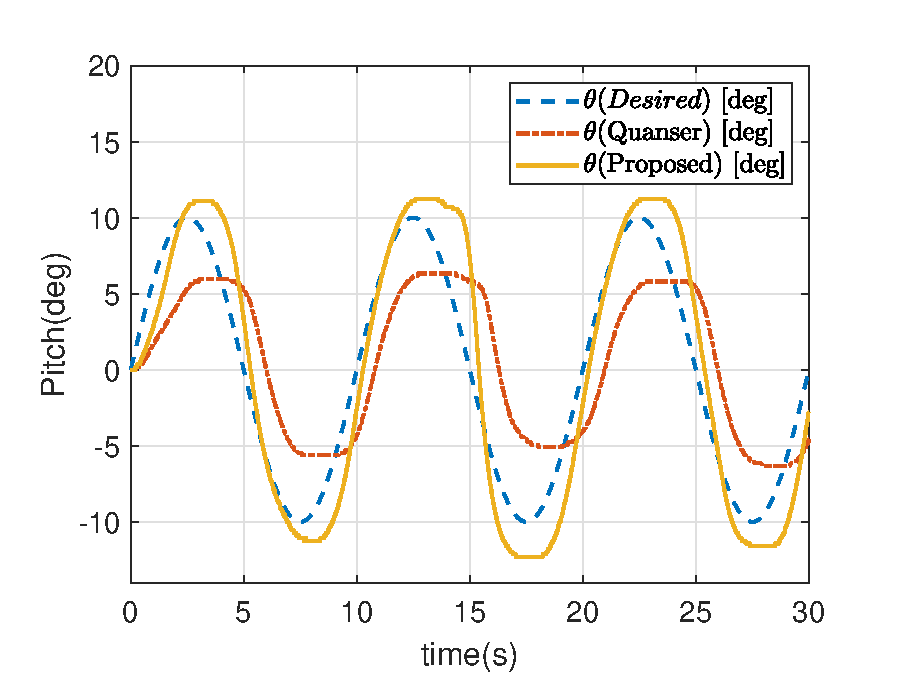
\includegraphics[width=.46\textwidth,keepaspectratio=true]{figs/matlab/LQR_PIvLQR_P_USB/sine/Pitch_LQR_RMSE.eps}
    \label{fig:Pitch_LQR_RMSE_Sine}
    }
    \subfigure[][]{
    \includegraphics[width=.46\textwidth,keepaspectratio=true]{figs/matlab/LQR_PIvLQR_P_USB/sine/Yaw_LQR_RMSE.eps}
    \label{fig:Yaw_LQR_RMSE_Sine}
    }    
    \subfigure[][]{
    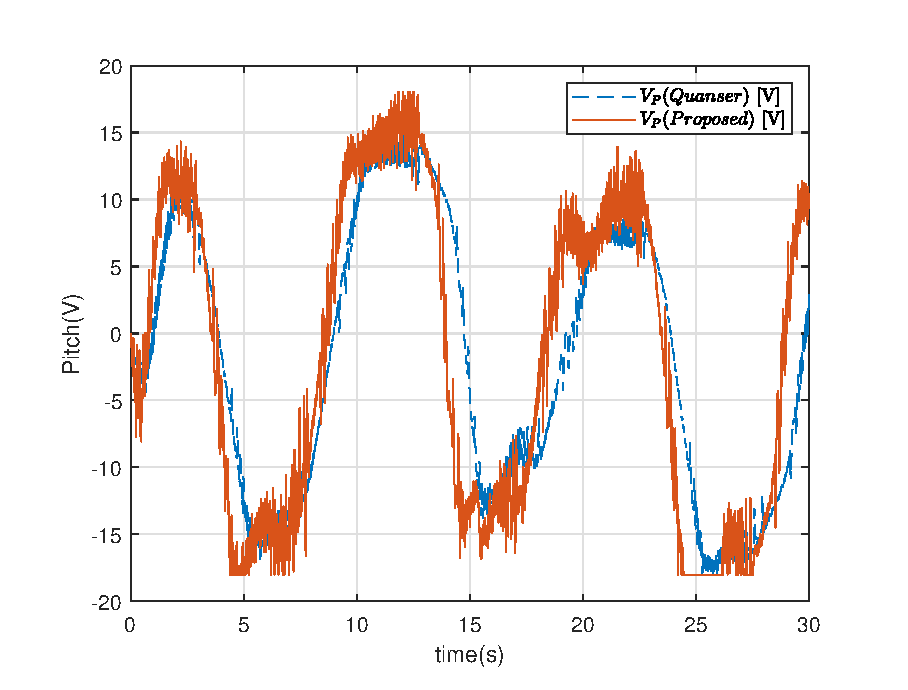
\includegraphics[width=.46\textwidth,keepaspectratio=true]{figs/matlab/LQR_PIvLQR_P_USB/sine/PitchVoltage_LQR_RMSE.eps}
    \label{fig:PitchVoltage_LQR_RMSE_Sine}
    }    
    \subfigure[][]{
    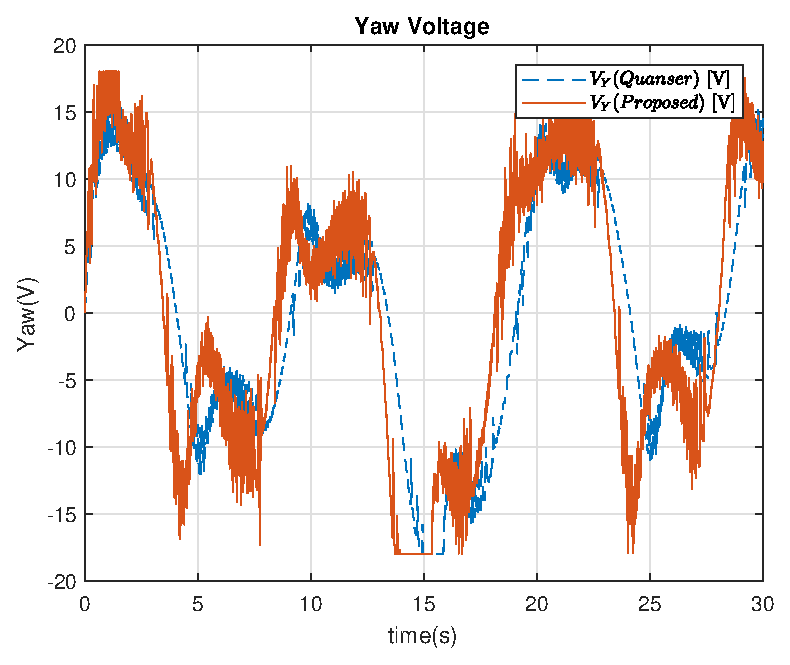
\includegraphics[width=.46\textwidth,keepaspectratio=true]{figs/matlab/LQR_PIvLQR_P_USB/sine/YawVoltage_LQR_RMSE.eps}
    \label{fig:YawVoltage_LQR_RMSE_Sine}
    }
    \subfigure[][]{
    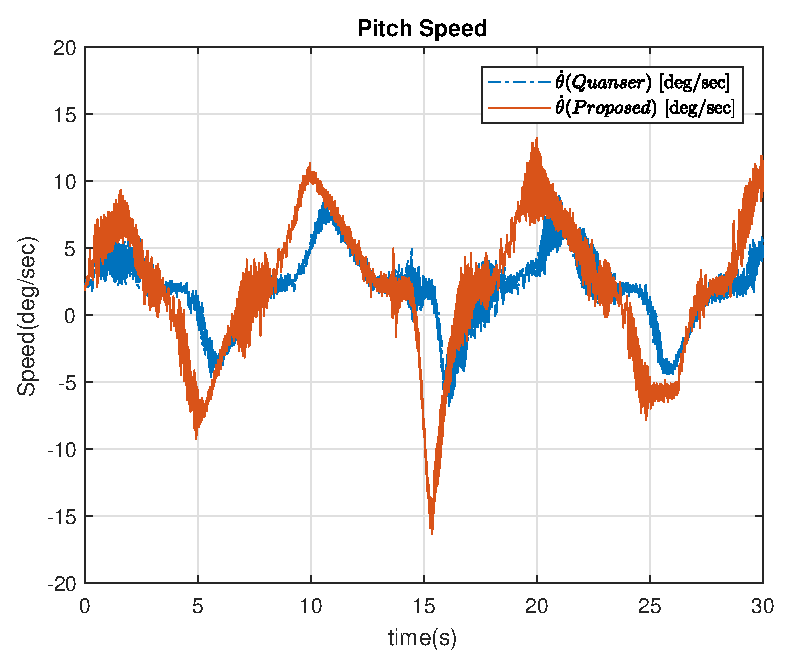
\includegraphics[width=.46\textwidth,keepaspectratio=true]{figs/matlab/LQR_PIvLQR_P_USB/sine/PitchSpeed_LQR_RMSE.eps}
    \label{fig:PitchSpeed_LQR_RMSE_Sine}
    }
    \subfigure[][]{
    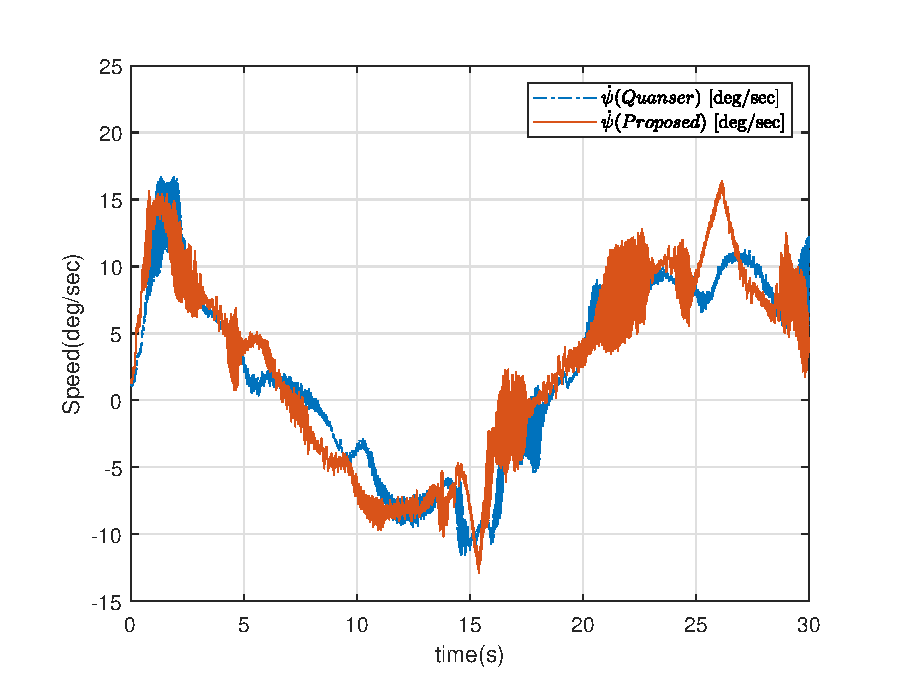
\includegraphics[width=.46\textwidth,keepaspectratio=true]{figs/matlab/LQR_PIvLQR_P_USB/sine/YawSpeed_LQR_RMSE.eps}
    \label{fig:PitchSpeed_LQR_RMSE_Sine}
    }
    \caption{USB implementation for proportional controller and proportional-integral controller calculated by LQR with a sinusoidal input.}
\end{figure}
%----------------------------------------------------------------------
\subsection{LQG (PI Controller)}
%----------------------------------------------------------------------

%----------------------------------------------------------------------
\subsection{ADP}
%----------------------------------------------------------------------



%----------------------------------------------------------------------
\subsection{Conclusions}
%----------------------------------------------------------------------
Note: constant used pitch 10 degrees, yaw 45 degrees\\
Note: square used pitch XXXX degrees with period of XXXX, yaw XXXX degrees with period of XXXX\\
Note: sine used pitch XXXX degrees with period of XXXX, yaw XXXX degrees with period of XXXX\\
\begin{table}[h!]
    \centering
    \begin{tabular}{l|l|l|l|l|l|l}
        \toprule
        \textbf{} & \textbf{LQR(P)} & \textbf{LQR(PI)} &
        \textbf{ADP(P)} \\
        \toprule
        RMSE Pitch Step & 2.6454 & ? & 1.3067 \\
        RMSE Yaw Step & 5.7991 & ? & 6.1991 \\
        RMSE Pitch Square & ? & ? & ? \\
        RMSE Yaw Square & ? & ? & ? \\
        RMSE Pitch Sine & ? & ? & ? \\
        RMSE Yaw Sine & ? & ? & ? \\
        \bottomrule
    \end{tabular}
    \caption{Error Comparison for USB Algorithms}
    \label{tab:USB_RMSE}
\end{table}
Based on the results XXXX preformed better for USB.
%----------------------------------------------------------------------

%======================================================================
\section{Raspberry Pi}

%----------------------------------------------------------------------
\subsection{LQR (P Controller)}
%----------------------------------------------------------------------

%----------------------------------------------------------------------
\subsection{ADP}
%----------------------------------------------------------------------

%----------------------------------------------------------------------
\subsection{Conclusions}
%----------------------------------------------------------------------
Note: constant used pitch XXXX degrees, yaw XXXX degrees\\
Note: square used pitch XXXX degrees with period of XXXX, yaw XXXX degrees with period of XXXX\\
Note: sine used pitch XXXX degrees with period of XXXX, yaw XXXX degrees with period of XXXX\\
\begin{table}[h!]
    \centering
    \begin{tabular}{l|l|l|l|l|l|l}
        \toprule
        \textbf{} & \textbf{LQR(P)} & \textbf{ADP(P)} \\
        \toprule
        RMSE Pitch Step & ? & ?  \\
        RMSE Yaw Step & ? & ? \\
        RMSE Pitch Square & ? & ? \\
        RMSE Yaw Square & ? & ? \\
        RMSE Pitch Sine & ? & ? \\
        RMSE Yaw Sine & ? & ? \\
        \bottomrule
    \end{tabular}
    \caption{Error Comparison for USB Algorithms}
    \label{tab:USB_RMSE}
\end{table}
Based on the results XXXX preformed better for Raspberry Pi.
%----------------------------------------------------------------------

%======================================================================
\section{Mobile Device}

%----------------------------------------------------------------------
\subsection{LQR (P Controller)}
%----------------------------------------------------------------------
\begin{figure}
    \centering
    \subfigure[][]{
    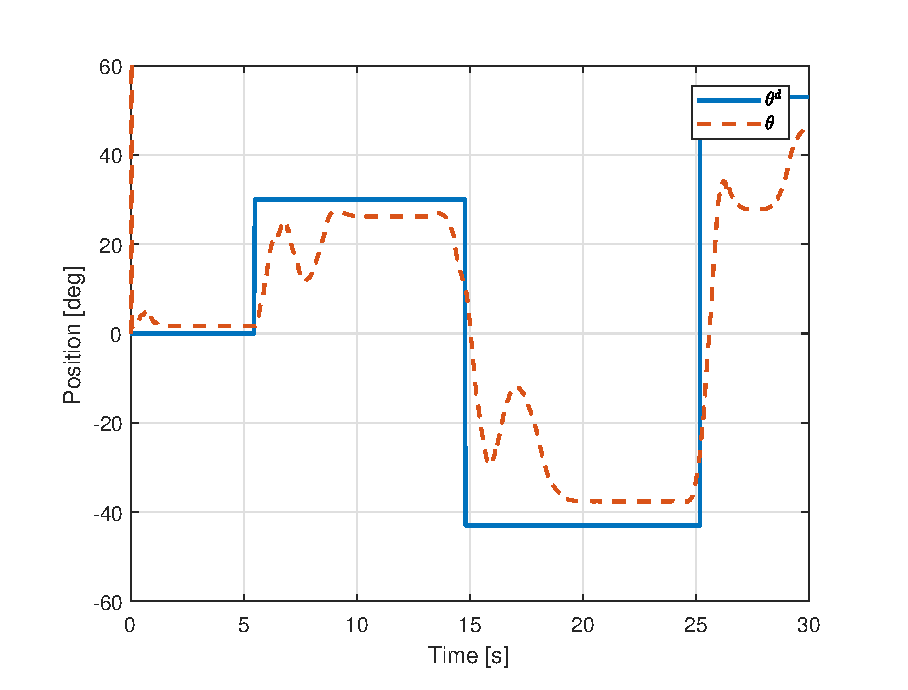
\includegraphics[width=.46\textwidth,keepaspectratio=true]{figs/matlab/LQR/P_Android/LQR_Pitchpos.eps}
    \label{fig:AndroidLQRPitchpos}
    }
    \subfigure[][]{
    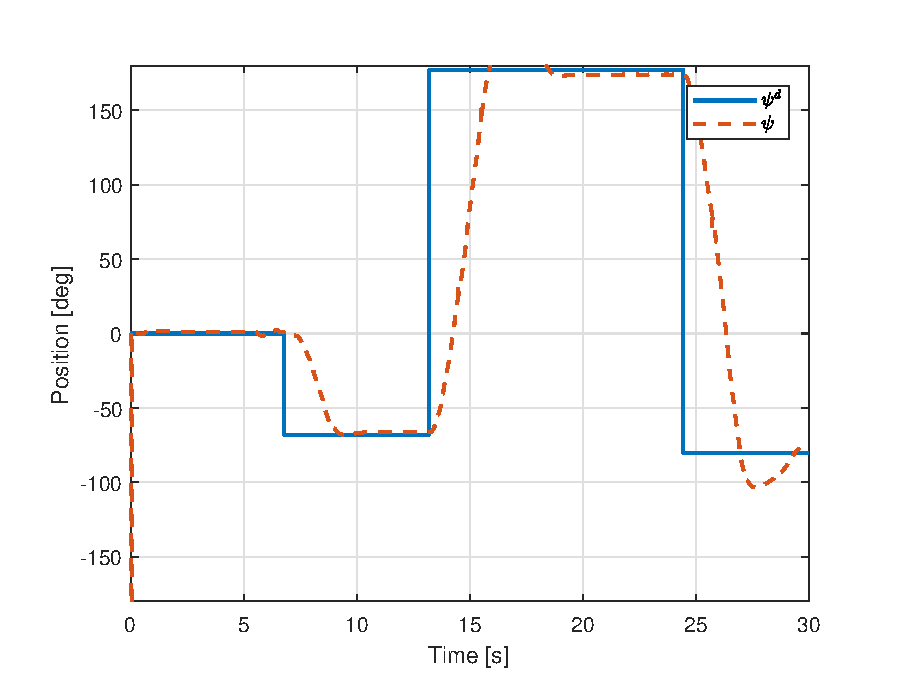
\includegraphics[width=.46\textwidth,keepaspectratio=true]{figs/matlab/LQR/P_Android/LQR_Yawpos.eps}
    \label{fig:AndroidLQRYawpos}
    }
    \subfigure[][]{
    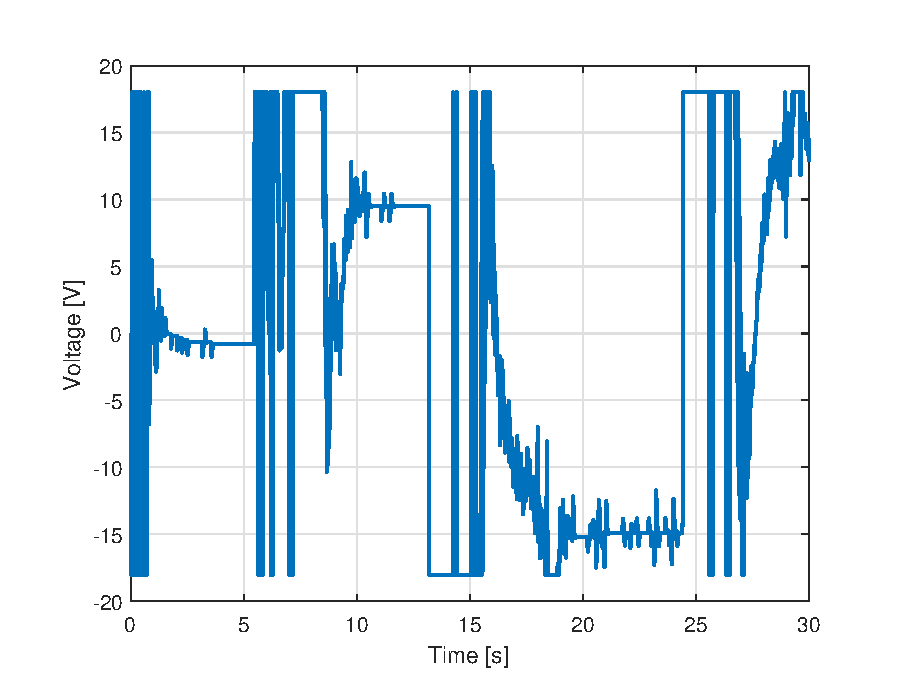
\includegraphics[width=.46\textwidth,keepaspectratio=true]{figs/matlab/LQR/P_Android/LQR_PitchVolt.eps}
    \label{fig:AndroidLQRPitchVolt}
    }
    \subfigure[][]{
    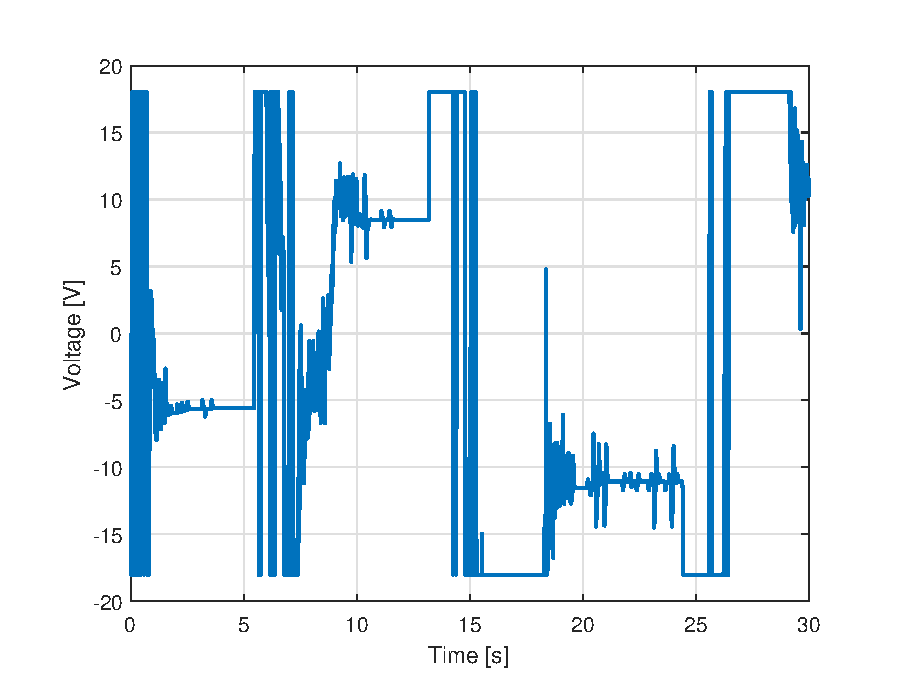
\includegraphics[width=.46\textwidth,keepaspectratio=true]{figs/matlab/LQR/P_Android/LQR_YawVolt.eps}
    \label{fig:AndroidLQRYawVolt}
    }
    \caption{LQR Android Results}
    \label{fig:AndroidLQR}
\end{figure}


%----------------------------------------------------------------------
\subsection{ADP}
%----------------------------------------------------------------------

\begin{figure}
    \centering
    \subfigure[][]{
    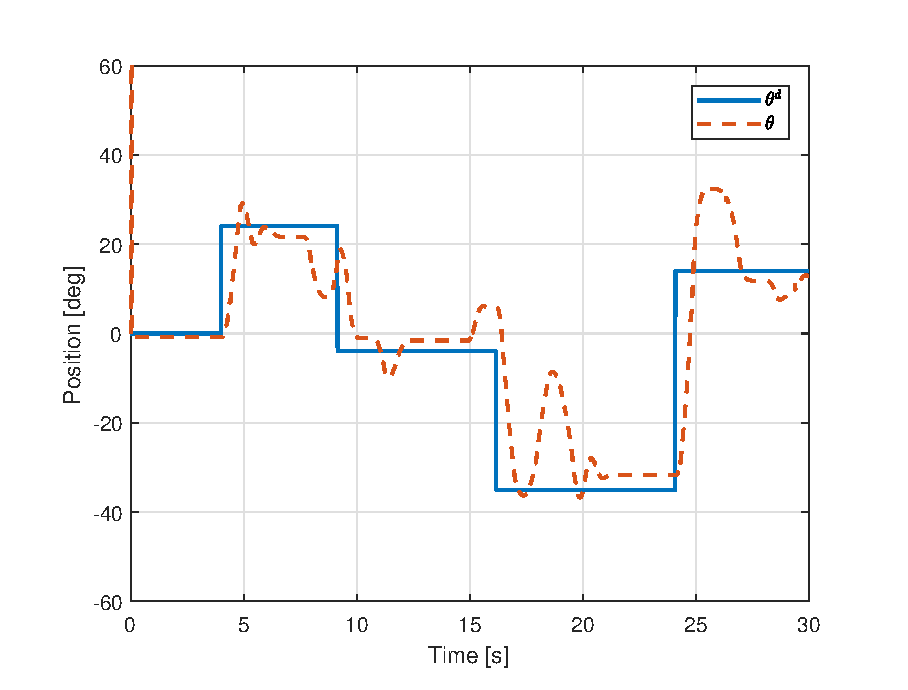
\includegraphics[width=.46\textwidth,keepaspectratio=true]{figs/matlab/ADP/Android/ADP_Pitch_Wireless.eps}
    \label{fig:AndroidADPPitchpos}
    }
    \subfigure[][]{
    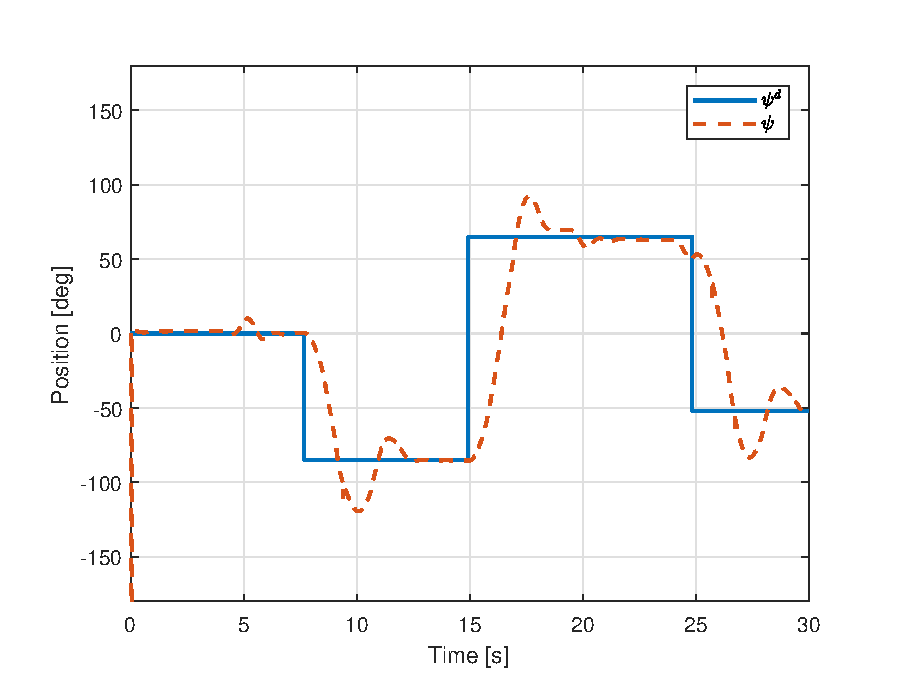
\includegraphics[width=.46\textwidth,keepaspectratio=true]{figs/matlab/ADP/Android/ADP_Yaw_Wireless.eps}
    \label{fig:AndroidADPYawpos}
    }
    \subfigure[][]{
    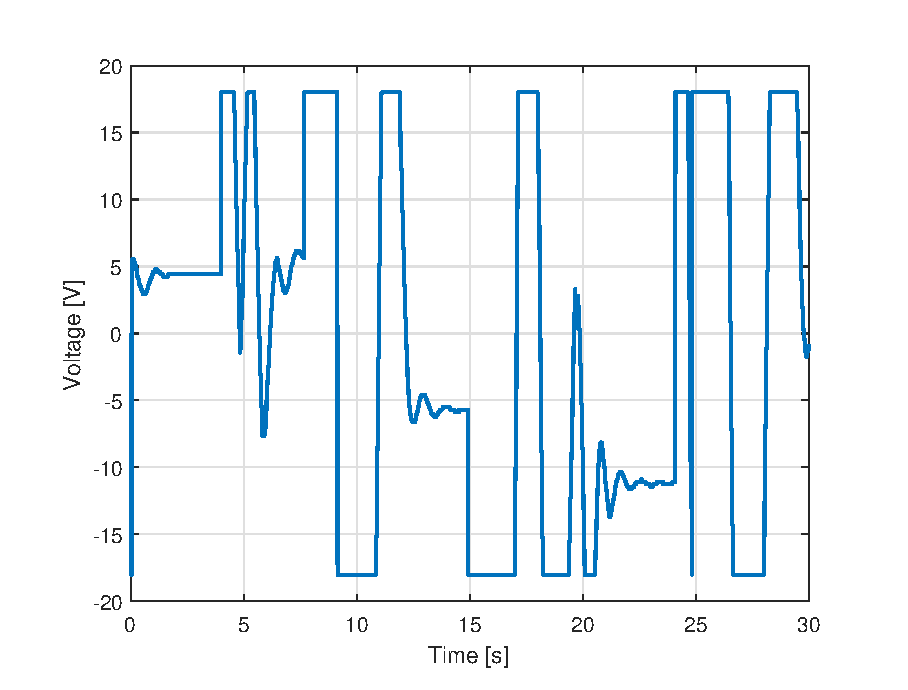
\includegraphics[width=.46\textwidth,keepaspectratio=true]{figs/matlab/ADP/Android/ADP_Pitch_Volt_Wireless.eps}
    \label{fig:AndroidADPPitchVolt}
    }
    \subfigure[][]{
    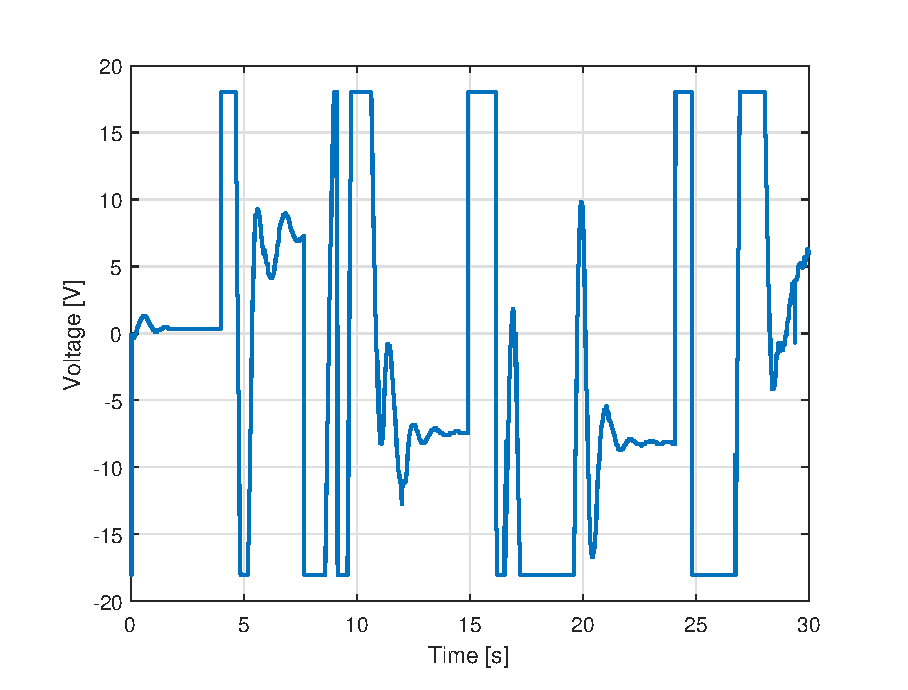
\includegraphics[width=.46\textwidth,keepaspectratio=true]{figs/matlab/ADP/Android/ADP_Yaw_Volt_Wireless.eps}
    \label{fig:AndroidADPYawVolt}
    }
    \caption{ADP Android Results}
    \label{fig:AndroidADP}
\end{figure}

%----------------------------------------------------------------------
\subsection{Conclusions}
%----------------------------------------------------------------------
Note: constant used pitch XXXX degrees, yaw XXXX degrees\\
Note: square used pitch XXXX degrees with period of XXXX, yaw XXXX degrees with period of XXXX\\
Note: sine used pitch XXXX degrees with period of XXXX, yaw XXXX degrees with period of XXXX\\
\begin{table}[h!]
    \centering
    \begin{tabular}{l|l|l|l|l|l|l}
        \toprule
        \textbf{} & \textbf{LQR(P)} & \textbf{ADP(P)} \\
        \toprule
        RMSE Pitch Step & ? & ?  \\
        RMSE Yaw Step & ? & ? \\
        RMSE Pitch Square & ? & ? \\
        RMSE Yaw Square & ? & ? \\
        RMSE Pitch Sine & ? & ? \\
        RMSE Yaw Sine & ? & ? \\
        \bottomrule
    \end{tabular}
    \caption{Error Comparison for USB Algorithms}
    \label{tab:USB_RMSE}
\end{table}
Based on the results XXXX preformed better for Android.

%----------------------------------------------------------------------


%%% Local Variables:
%%% mode: latex
%%% TeX-master: "../finalReport"
%%% End:

%======================================================================
\chapter{Conclusion and Future Work}
\label{ch: Chapter6}
%======================================================================

%----------------------------------------------------------------------
\section{Algorithm Comparison}
%----------------------------------------------------------------------

%----------------------------------------------------------------------
\section{Conclusion}
%----------------------------------------------------------------------

%----------------------------------------------------------------------
\section{Future Work}
%----------------------------------------------------------------------
\subsection{Enhanced Smart Framework}
\begin{figure}[!htbp]
    \centering
    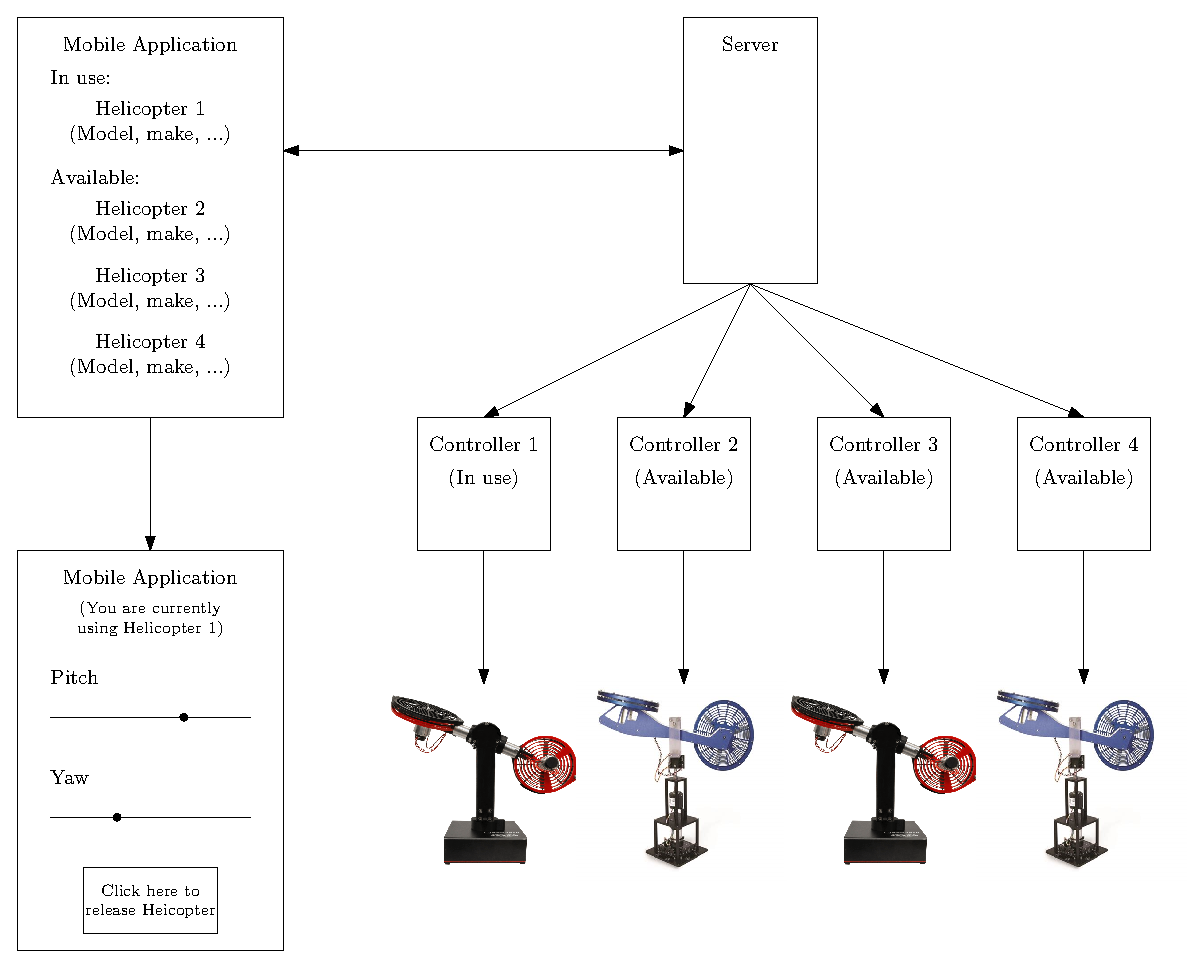
\includegraphics[width=.46\textwidth,keepaspectratio=true]{figs/ipe/smartAlg.eps}
    \label{fig:Smart_Alg}
    \caption{Smart Algorithm Server Connectivity}
\end{figure}

\subsection{Digital Compass}

\subsection{Expanded PI Control}
We had trouble implementing the PI control architecture as well as LQG on the Raspberry Pi. This may be because the integrator and the kalman filter require a fixed sampling time.  Simulink has the option to use a variable sampling time when set to continuous time.  Since the model is being loaded onto a embedded system which relies upon a fixed sampling time, this may be affected the values being outputted by these blocks.\\
To correct this issue, we recommend that future work done on this project convert the model to discrete time.  Consider \ref{eq:discreteA} and \ref{eq:discreteB} to convert the continuous model in \ref{eq:stateModel}:
\begin{equation}
\label{eq:discreteA}
    x(k+1)=\Phi x(k)+\Gamma u(k)
\end{equation}
\begin{equation}
\label{eq:discreteB}
    y(k)=Hx(k)+Ju(k)
\end{equation}
where $T$ is the sampling time, $\Phi=e^{AT}$, and $\Gamma=\int_0^T e^{A\eta} d\eta B$.
%----------------------------------------------------------------------



%%% Local Variables:
%%% mode: latex
%%% TeX-master: "../finalReport"
%%% End:


% %----------------------------------------------------------------------
% % APPENDICES
% %---------------------------------------------------------------------- 
\appendix
% % Designate with \appendix declaration which just changes numbering style 
% % from here on
% % Add a title page before the appendices and a line in the Table of Contents
\addcontentsline{toc}{chapter}{APPENDICES} 
% %

%======================================================================
\chapter{Parameters and State-Space}
\label{ch: AppendixA}
%======================================================================

%----------------------------------------------------------------------
\section{Parameters}

\begin{figure}[!htbp]
 \begin{center}
  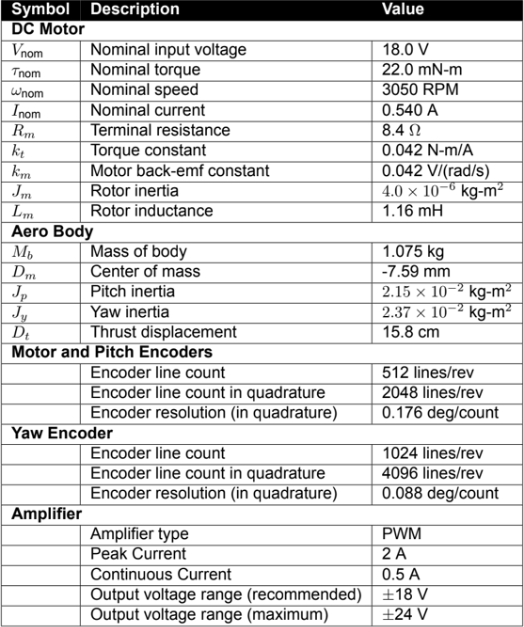
\includegraphics[scale=.75]{figs/img/quanserAeroSystemParameters}
 \end{center}
\caption{System parameters used for the Quanser Aero.}
\label{fig.systemParameters}
\end{figure}

\lstinputlisting{code/simulation/quanser_aero_parameters.m}
%----------------------------------------------------------------------

%----------------------------------------------------------------------
\section{State-Space Model}
\lstinputlisting{code/simulation/quanser_aero_state_space.m}
%----------------------------------------------------------------------



%%% Local Variables:
%%% mode: latex
%%% TeX-master: "../finalReport"
%%% End:

%======================================================================
\chapter{MATLAB Simulation Code}
%======================================================================

%----------------------------------------------------------------------
\section{LQR (P controller)}
\label{ch:codeLQRsim}
\lstinputlisting{parts/MATLAB_Code/KV_LQRContinuousTime.m}
%----------------------------------------------------------------------

%----------------------------------------------------------------------
\section{LQR (PI controller)}
%----------------------------------------------------------------------

%----------------------------------------------------------------------
\section{LQG (PI Controller)}
%----------------------------------------------------------------------


%%% Local Variables:
%%% mode: latex
%%% TeX-master: "../finalReportMainV1"
%%% End:

%%======================================================================
\chapter{USB MATLAB Code}
%======================================================================

%----------------------------------------------------------------------
%\section{New Section}
%----------------------------------------------------------------------


%%% Local Variables:
%%% mode: latex
%%% TeX-master: "../finalReportMainV1"
%%% End:

%======================================================================
\chapter{Raspberry Pi MATLAB Code}
%======================================================================

%----------------------------------------------------------------------
\section{}
%----------------------------------------------------------------------


%----------------------------------------------------------------------
\section{Initialization Code}
\label{ch:RPI3_SPI_Int}
\lstinputlisting{parts/MATLAB_Code/RPI3_SPI_Int.m}


%----------------------------------------------------------------------
%%% Local Variables:
%%% mode: latex
%%% TeX-master: "../finalReportMainV1"
%%% End:

%======================================================================
\chapter{ADP MATLAB Code}
%======================================================================

%----------------------------------------------------------------------
\section{Initialization Code}
%----------------------------------------------------------------------
\label{ch:RPI3_SPI_Int}
\lstinputlisting{code/implementation/ADP/raspberry/ADP_Init.m}

%----------------------------------------------------------------------
\section{Update Weights}
%----------------------------------------------------------------------
\label{ch:RPI3_SPI_Int}
\lstinputlisting{code/implementation/ADP/quanserAEROCriticTuning.m}


%----------------------------------------------------------------------
%%% Local Variables:
%%% mode: latex
%%% TeX-master: "../finalReportMainV1"
%%% End:

%======================================================================
\chapter{Tutorials}
%======================================================================

%----------------------------------------------------------------------
\section{USB Connection}
%----------------------------------------------------------------------
\begin{enumerate}
    \item Verify QuaRC is installed on computer
    \item Install QFLEX 2 USB into Quanser Aero as seen in Figure~\ref{fig:USB_Panel}
    \item Open Simulink model
    \item Connect Quanser Aero to computer via the included USB adapter cable
    \item Set simulation mode to external
    \item Run MATLAB initialization code for motion controller
    \item Click "Build Model" button
    \item Click "Connect To Target" button
    \item Click "Run" button
\end{enumerate}

\begin{figure}[!h]
    \centering
    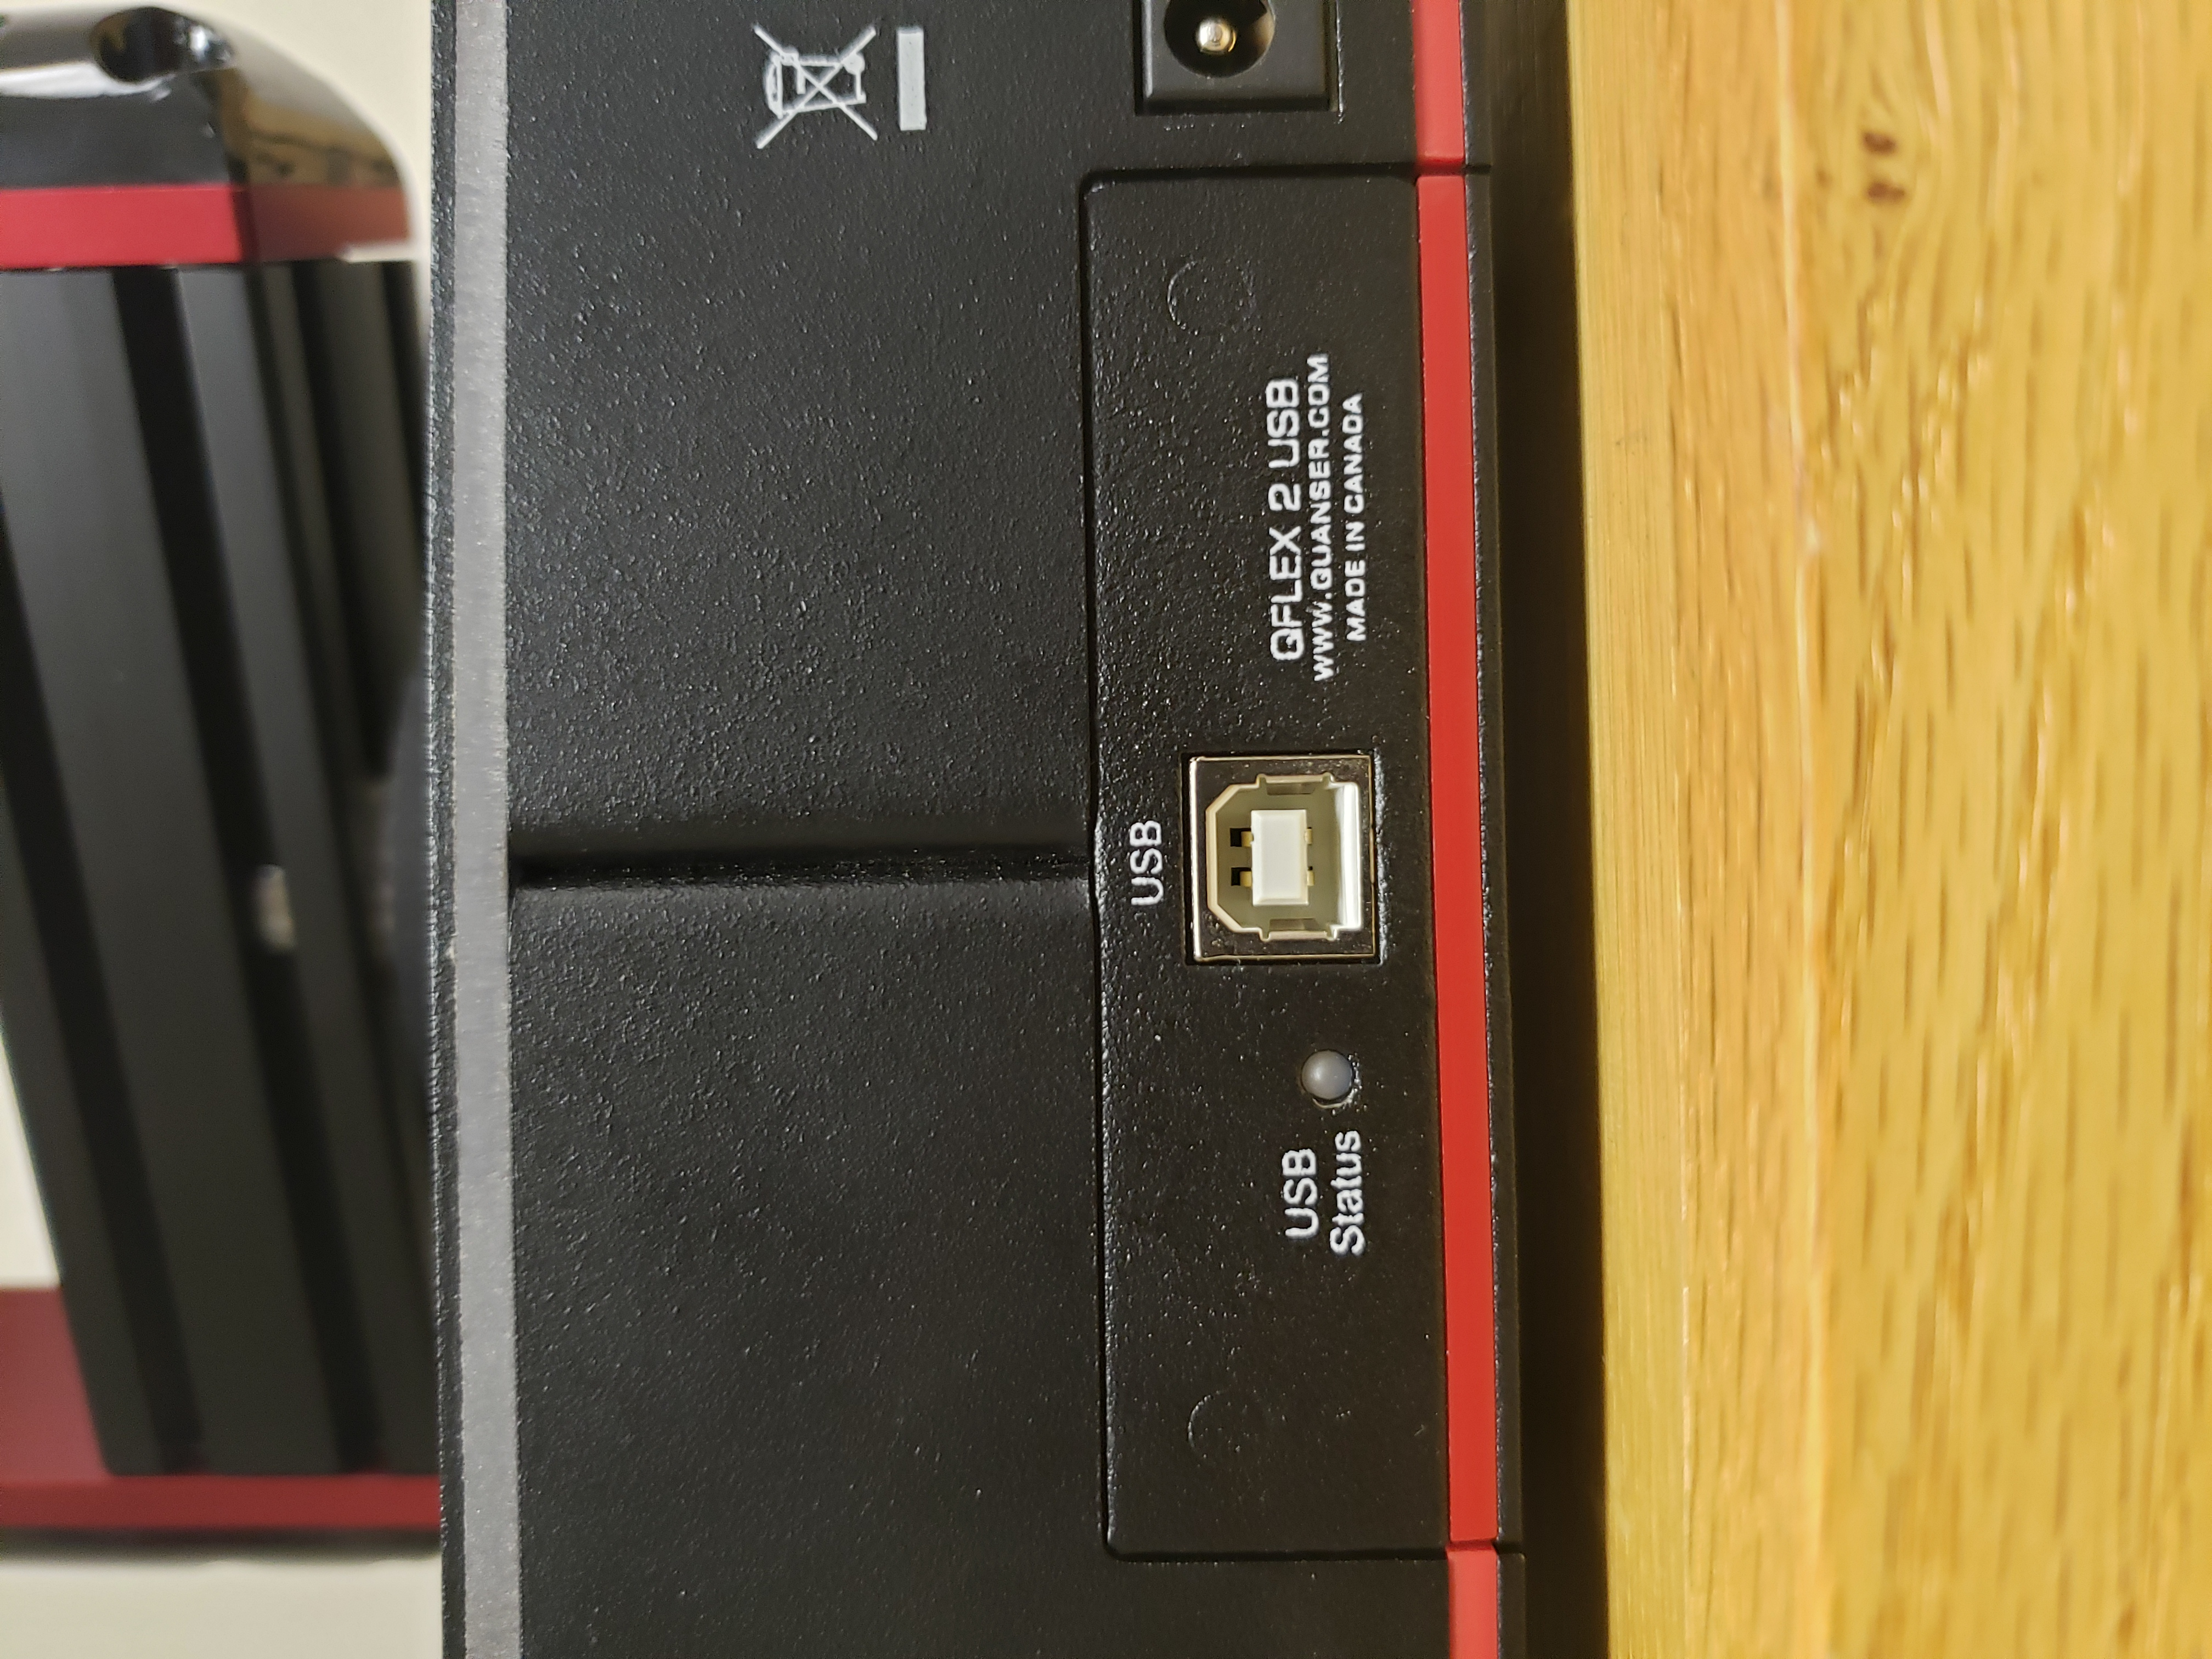
\includegraphics[angle = 270,width=.248\textwidth,keepaspectratio=true]{figs/img/USB_Panel.jpg}
    \label{fig:USB_Panel}
    \caption{Quanser Aero with QFLEX 2 USB panel installed}
\end{figure}
%----------------------------------------------------------------------
\section{Raspberry Pi Implementation}
%----------------------------------------------------------------------
\begin{enumerate}
    \item Make sure software add ons are installed on MATLAB
    \begin{enumerate}
        \item MATLAB Support Package for Raspberry Pi Hardware
        \item Simulink Support Package for Raspberry Pi Hardware
    \end{enumerate}
    \item Install QFLEX 2 Embedded into Quanser Aero as seen in Figure~\ref{fig:Embedded_Panel}
    \item Assuming Raspberry PI is not connected to network, establish a serial connection to the Raspberry PI
    \item \todo[inline]{Setup Raspberry PI on the network}
    \item Connect SPI wires to Raspberry PI. Pin 1 (white wire) on the embedded panel connects to +5V on the Pi.  Pin 2 (yellow wire) connects to GPIO 10 on the Pi. Pin 3 (blue wire) connects to GPIO 9 on the Pi.  Pin 4 (green wire) connects to GPIO 11 on the Pi. Pin 6 (purple wire) connects to GPIO 8 on the Pi.  Pin 7 (Red wire) connects to ground on the Pi.
    \item Connect Raspberry PI to QFLEX 2 Embedded
    \item Right click on Simulink model
    \item Open "Model Configuration Parameters"
    \item Select "Hardware Implementation"
    \item Set "Hardware Board" to "Raspberry Pi"
    \item Under "Board Parameters" under "Groups" type in the IP address of the Raspberry PI, the username, and password
    \item Under "Build options", set build action to "Build and run" and type in the file path that you want the model to be stored on the Raspberry PI
    \item Set simulation mode to external
    \item Run MATLAB initialization code for motion controller
    \item Run MATLAB Raspberry PI/SPI initialization code \ref{ch:RPI3_SPI_Int}
    \item Click "Deploy to Hardware" button
    \item To stop program you must "kill" it
    \item Open Putty, connect to your Raspberry PI, and log in
    \item Type "ps -A" to view running programs and find the process number of your Simulink model
    \item Type "sudo kill -9 \#\#\#\#" where \#\#\#\# is your process number.  This will kill the program
\end{enumerate}

\begin{figure}[!h]
    \centering
    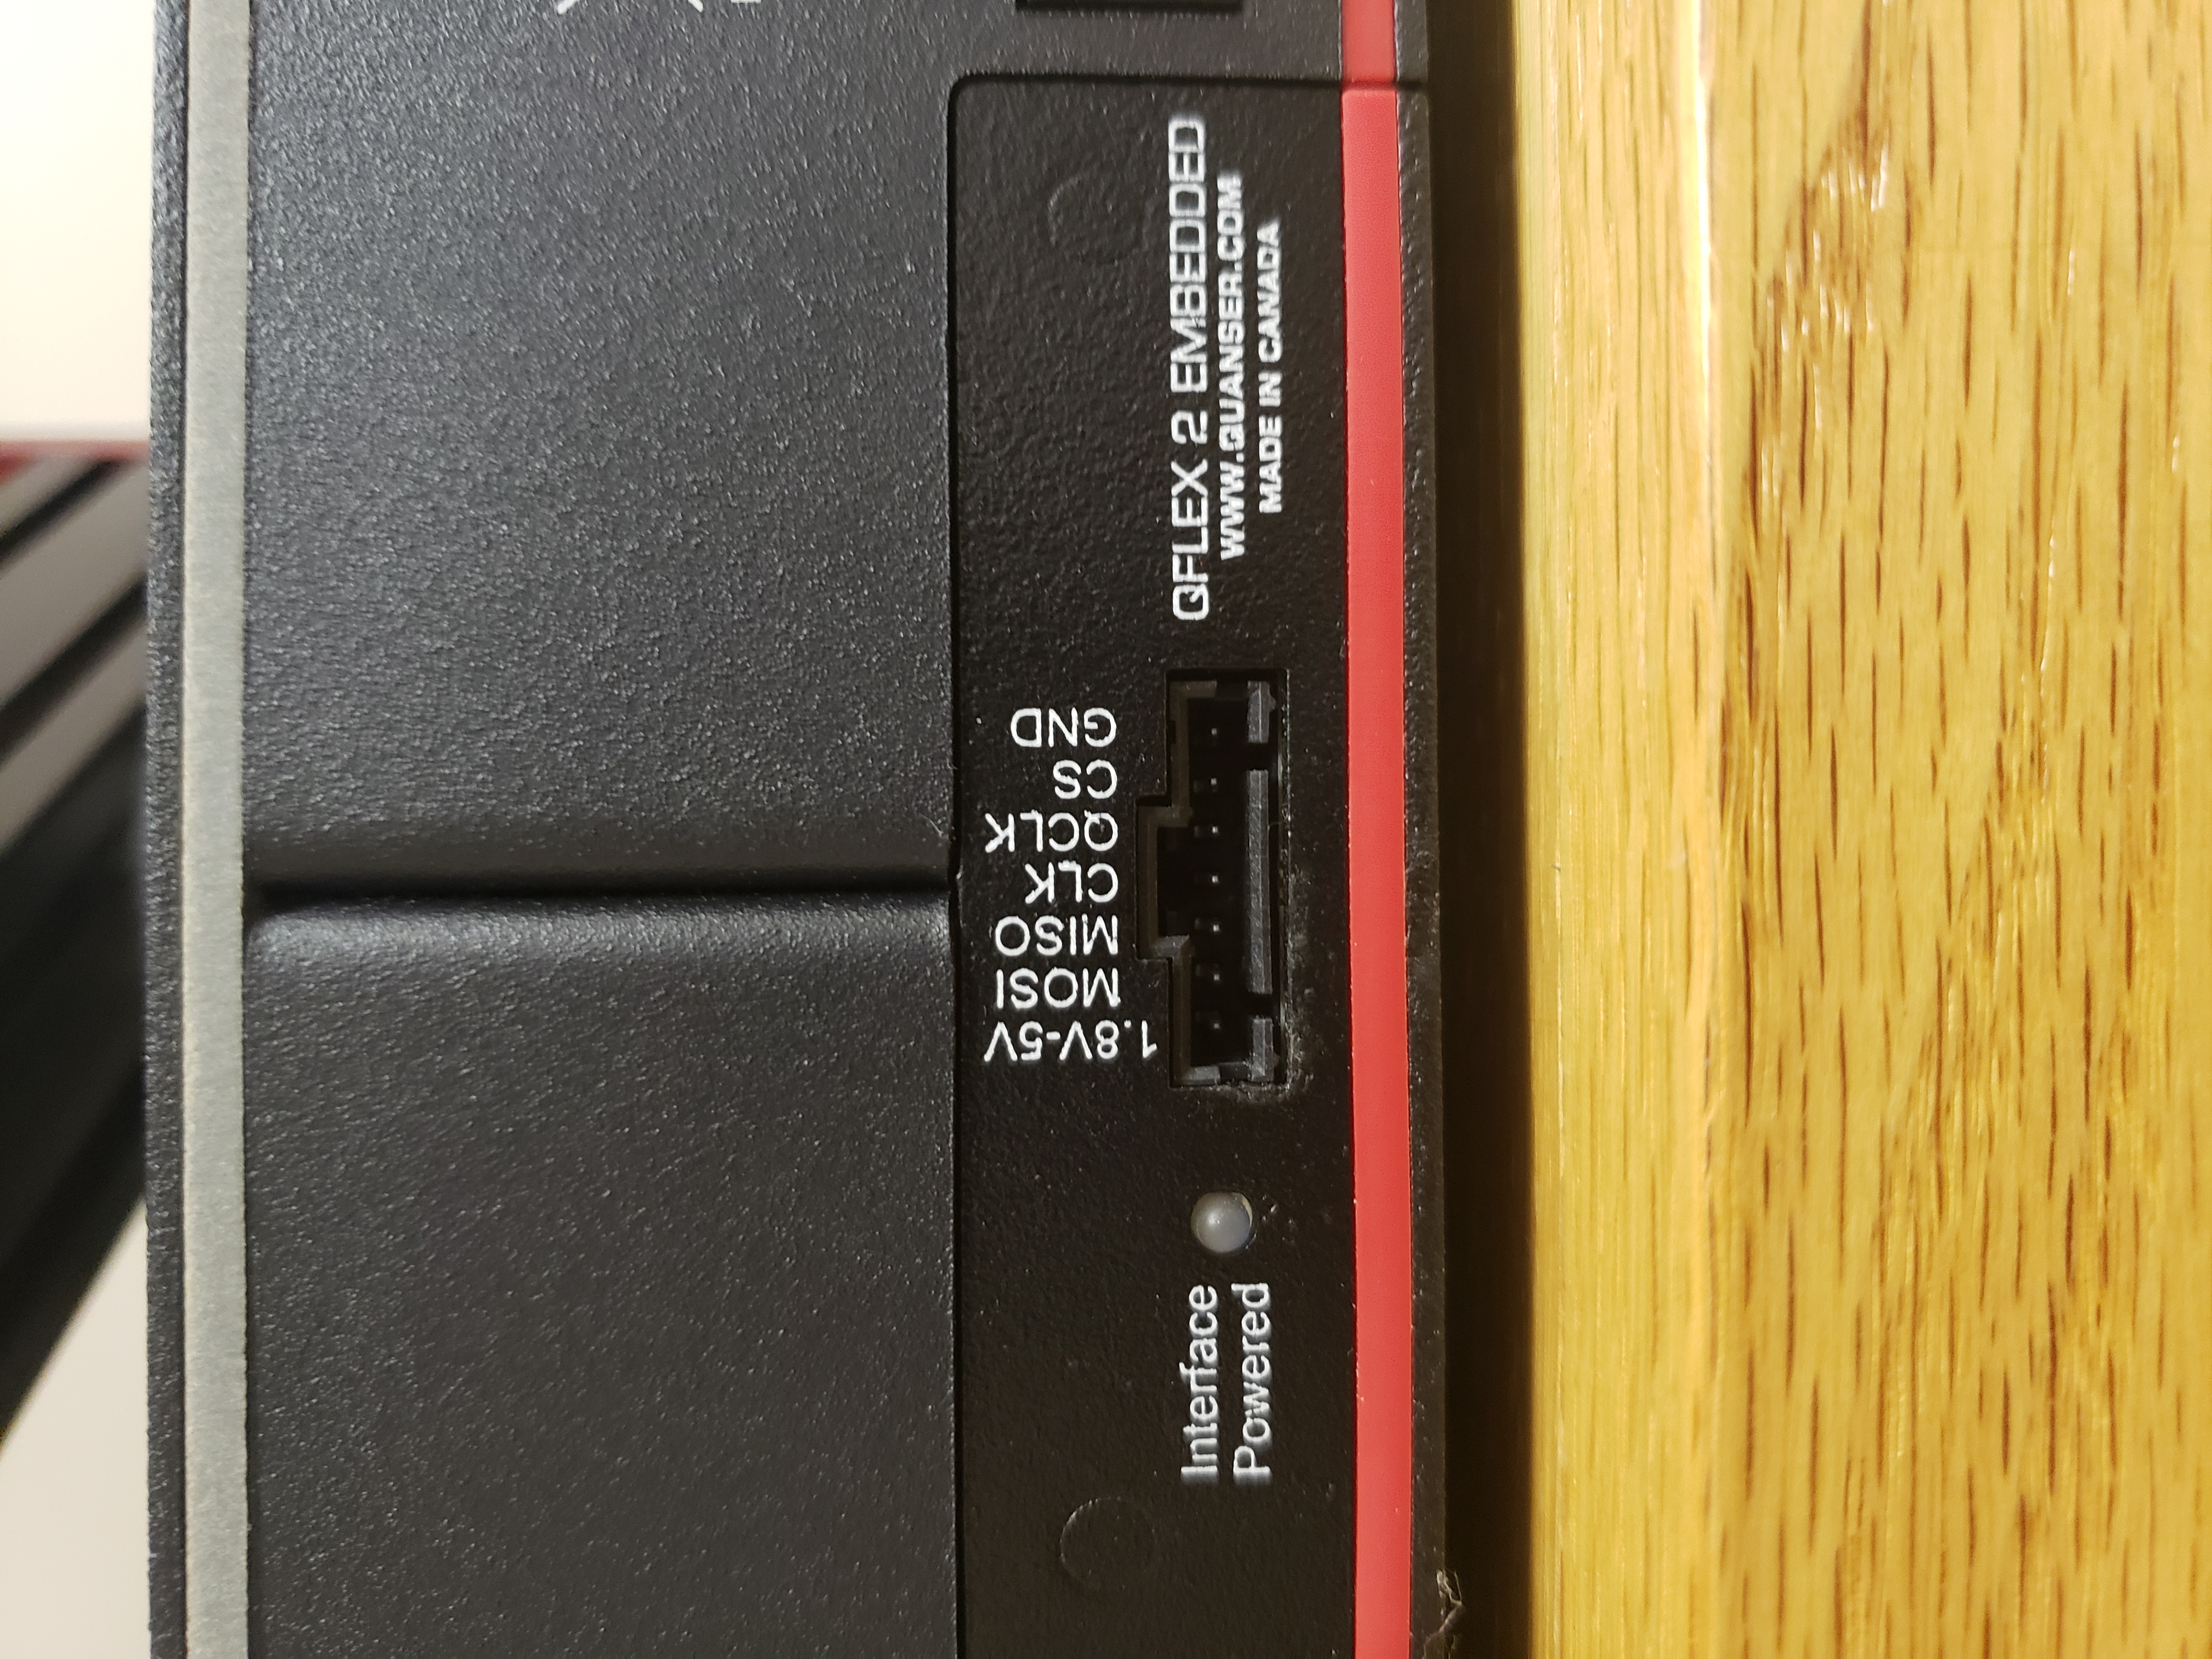
\includegraphics[angle = 270,width=.248\textwidth,keepaspectratio=true]{figs/img/Embedded_Panel.jpg}
    \label{fig:Embedded_Panel}
    \caption{Quanser Aero with QFLEX 2 Embedded panel installed}
\end{figure}
%----------------------------------------------------------------------
\section{Android Application}
%----------------------------------------------------------------------


%%% Local Variables:
%%% mode: latex
%%% TeX-master: "../finalReport"
%%% End:


%% An appendix
%======================================================================
\chapter{Sources of Information and Help}
\label{ch:Appendix-Sources-of-Info}
%======================================================================
The best source of information about \LaTeX\ is the two books mentioned in this course \cite{lamport.book,goossens.book}.
Another excellent resource is the UseNet newsgroup \verb=comp.text.tex=.
A frequently-asked-questions (FAQ) list is also maintained by this news group.
You might also search the World Wide Web for ``LaTeX'' for other sources of help.


%%% Local Variables:
%%% mode: latex
%%% TeX-master: "../finalReportMainV1"
%%% End:
 %"Sources of Information and Help"
%% An appendix
%======================================================================
\chapter[PDF Plots From Matlab]{Matlab Code for Making a PDF Plot}
\label{ch:Appendix-Matlab} 
%======================================================================
\section{Using the GUI}
Properties of Matab plots can be adjusted from the plot window via a graphical interface. Under the Desktop menu in the Figure window, select the Property Editor. You may also want to check the Plot Browser and Figure Palette for more tools. To adjust properties of the axes, look under the Edit menu and select Axes Properties.

To set the figure size and to save as PDF or other file formats, click the Export Setup button in the figure Property Editor.

\section{From the Command Line} 
All figure properties can also be manipulated from the command line. Here's an example: 
\begin{verbatim}
x=[0:0.1:pi];
hold on % Plot multiple traces on one figure
plot(x,sin(x))
plot(x,cos(x),'--r')
plot(x,tan(x),'.-g')
title('Some Trig Functions Over 0 to \pi') % Note LaTeX markup!
legend('{\it sin}(x)','{\it cos}(x)','{\it tan}(x)')
hold off
set(gca,'Ylim',[-3 3]) % Adjust Y limits of "current axes"
set(gcf,'Units','inches') % Set figure size units of "current figure"
set(gcf,'Position',[0,0,6,4]) % Set figure width (6 in.) and height (4 in.)
cd n:\thesis\plots % Select where to save
print -dpdf plot.pdf % Save as PDF
\end{verbatim} 


%%% Local Variables:
%%% mode: latex
%%% TeX-master: "../finalReportMainV1"
%%% End:
 %"Matlab Code for Making a PDF Plot"

% %----------------------------------------------------------------------
% % END MATERIAL
% %----------------------------------------------------------------------

% % B I B L I O G R A P H Y
% % -----------------------
% %
% % The following statement selects the style to use for references.  It controls the sort order of the entries in the bibliography and also the formatting for the in-text labels.
\bibliographystyle{plain}
% % This specifies the location of the file containing the bibliographic information.  
% % It assumes you're using BibTeX (if not, why not?).
% \ifthenelse{\boolean{PrintVersion}}{
% \cleardoublepage % This is needed if the book class is used, to place the anchor in the correct page,
%                  % because the bibliography will start on its own page.
% }{
% \clearpage       % Use \clearpage instead if the document class uses the "oneside" argument
% }
% \phantomsection  % With hyperref package, enables hyperlinking from the table of contents to bibliography             
% % The following statement causes the title "References" to be used for the bibliography section:
% % \renewcommand*{\bibname}{References}
% Bibliography 
\renewcommand{\bibname}{Bibliography}

% Add the References to the Table of Contents
\addcontentsline{toc}{chapter}{\textbf{References}}

\bibliography{bib/refsHelicopter,bib/refsSuruzWeb}
% Tip 5: You can create multiple .bib files to organize your references. 
% Just list them all in the \bibliogaphy command, separated by commas (no spaces).


%----------------------------------------------------------------------
\end{document}
%======================================================================



%%% Local Variables: 
%%% mode: latex
%%% TeX-master: t
%%% End: 
